% template.tex, dated April 5 2013
% This is a template file for Annual Reviews 1 column Journals
%
% Compilation using ar-1col.cls' - version 1.0, Aptara Inc.
% (c) 2013 AR
%
% Steps to compile: latex latex latex
%
% For tracking purposes => this is v1.0 - Apr. 2013

\documentclass{ar-1col}

\usepackage{url}
\usepackage[numbers,sort&compress]{natbib}

%% added packages
\usepackage{xspace}
\usepackage{graphicx}
\usepackage{amssymb}
\usepackage{enumitem}
%\usepackage[top=2cm,bottom=3cm]{geometry}
\usepackage[svgnames]{xcolor}
% hyper-ref prevents the document from compiling on the arXiv - it is
% included in some other `usepackage` and that generates a conflict.
% Will attempt to use it differently, hope for a better outcome.
%\usepackage[bookmarks=false]{hyperref}
\usepackage[bookmarks=false,colorlinks=true,linkcolor=DarkBlue,citecolor=DarkBlue]{hyperref}
\usepackage{subfig}
%\usepackage{subcaption}
\usepackage{rotating}
\usepackage{units}
\usepackage{amsmath}
\usepackage{bm}     % nice math bold italics
\usepackage{lineno}
\usepackage{listings}
\usepackage{lmodern} % suppress font warnings
\usepackage[normalem]{ulem}
\usepackage[section]{placeins}
\usepackage{hepunits}
\usepackage{hepparticles}
\usepackage{cancel}
\usepackage{hepnames}
%\usepackage{epstopdf}
\usepackage{mathtools}
\usepackage[capitalise]{cleveref}
\usepackage{braket}
\usepackage{slashed}
%\usepackage{xcolor}
\usepackage{multirow}

\usepackage[Export]{adjustbox}

\providecommand{\cw}[1]{{\color{purple} Callum: #1}}
\newcommand\citeneeded{[{\color{blue} \underline{CITATION NEEDED}}]}
\newcommand{\change}[1]{{\color{red} #1}}
%\def\addcite#1{{\color{red}CITE[#1]}}
%\def\addcomment#1{{\color{red}COMMENT: #1}}
\def\asm#1{{\color{blue}#1}}
\def\del#1{}
\def\done#1{{\color{brown}#1}}
\definecolor{ao(english)}{rgb}{0.0, 0.5, 0.0}

% Greek letters
\def\g{\gamma}
\def\t{\tau}

\def\D{\Delta}
\def\G{\Gamma}
\def\O{\Omega}

% math
\makeatletter
\newcommand*\dotp{\mathpalette\bigcdot@{.5}}
\newcommand*\bigcdot@[2]{\mathbin{\vcenter{\hbox{\scalebox{#2}{$\m@th#1\bullet$}}}}}
\makeatother


\def\Dslash{D\hskip-0.65em /}
\def\Dslashe{D\hskip-0.5em /}
\def\tsep{t_{\rm sep}}
\def\tmin{t_{\rm min}}

%\newcommand{\Umunu}{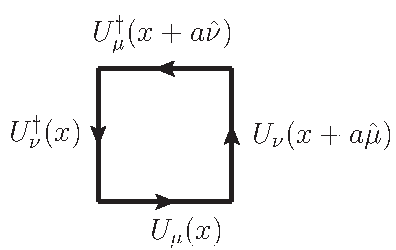
\includegraphics[width=0.5\textwidth,fbox=1pt,valign=c]{plots/plaquette}}
\newcommand{\Umunu}{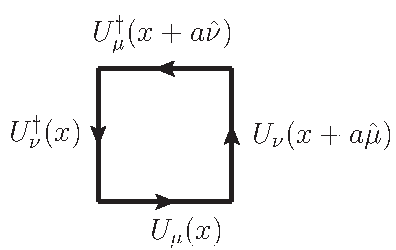
\includegraphics[width=0.6\textwidth,valign=c]{plots/plaquette}}

\setcounter{secnumdepth}{4}

% Metadata Information
\jname{Annu. Rev. Nucl. Part. Sci.}
\jvol{AA}
\jyear{2022}
\doi{10.1146/((please add article doi))}


% Document starts
\begin{document}

% Page header
\markboth{A. Meyer, A. Walker-Loud, C. Wilkinson}{LQCD relevance for the few-GeV neutrino program}

% Title
\title{Status of Lattice QCD Determination of Nucleon Form Factors
 and their Relevance for the Few-GeV Neutrino Program}

%Authors, affiliations address.
\author{Aaron S. Meyer$^{1,2}$,
Andr\'{e} Walker-Loud$^2$,
Callum Wilkinson$^3$
\affil{$^1$Department of Physics, University of California, Berkeley, CA, 94720, USA}
\affil{$^2$Nuclear Science Division, Lawrence Berkeley National Laboratory, Berkeley, CA, 94720, USA}
\affil{$^3$Physics Division, Lawrence Berkeley National Laboratory, Berkeley, CA, 94720, USA}
}

\begin{abstract}
Microscopic calculations of neutrino-nucleus cross sections begin with the neutrino-nucleon interaction\del{, making it}\asm{. This makes it} critically important to the interpretation of \del{neutrino-nucleus experiments, including }flagship \del{efforts to probe }neutrino oscillation\del{s} \asm{experiments}.
Yet, measurements of the single-nucleon interaction are limited and \asm{have}\del{of} poor statistics.
Alternatively, lattice QCD can be used to determine these interactions directly from the Standard Model with fully quantified theoretical uncertainties.
Recent lattice QCD results of $g_{\mathrm{A}}$ are in excellent agreement with experimental data,
and it is anticipated that results for the (quasi-)elastic nucleon form factors with full uncertainty budgets will be available within a \change{few} years.
We review the status of the field and lattice QCD results for the nucleon axial form factor, $F_{\mathrm{A}}(Q^2)$, a major source of uncertainty in modeling the neutrino-nucleon interaction for $E_{\nu} \lesssim 1$ GeV.
Results from different lattice calculations are in good agreement with each other, but collectively, in poor agreement with existing models of $F_{\mathrm{A}}(Q^2)$.
We discuss the potential impact of these lattice QCD results for current and future neutrino oscillation experiments.
We describe a road map to solidify confidence in the lattice results and discuss future calculations of more complicated processes, such as the resonant neutrino-nucleon reactions, which are important
to neutrino oscillation experiments in the few-GeV energy regime.
\end{abstract}

%Keywords, etc.
\begin{keywords}
Neutrino Oscillations, Nucleon Form Factors, Lattice QCD
%keywords, separated by comma, no full stop, lowercase
\end{keywords}

\maketitle

%Table of Contents
\tableofcontents


% ------------------------------------------------------------------------------
% Intoroduction
\section{Introduction\label{sec:intro}}

A major experimental program is underway which seeks to measure
as of yet unknown properties associated with the change of flavor of neutrinos.
In particular, the neutrino mass hierarchy and%
\begin{marginnote}
\entry{CP}{charge-parity}
\end{marginnote}%
CP violating phase
of neutrinos still remain to be measured, with additional focuses on measuring
oscillation parameters with high precision and testing whether the current
three-flavor mixing paradigm is sufficient~\cite{Esteban:2020cvm, ParticleDataGroup:2020ssz}.
These goals introduce stringent requirements on the precision of current and future experiments.
High-intensity beams are required to produce a sufficient flux of neutrinos to accumulate the necessary statistics.
Increased statistics place additional burden on our understanding of the systematic uncertainties needed for the experimental program.

Two\del{,} \done{large-scale}, next-generation experiments designed to meet these experimental constraints
are
%the Deep Underground Neutrino Experiment (DUNE)~\cite{Abi:2020wmh}
DUNE~\cite{Abi:2020wmh}
and
%Hyper-Kamiokande experiment (Hyper-K)~\cite{Hyper-Kamiokande:2018ofw}.
Hyper-K~\cite{Hyper-Kamiokande:2018ofw}.
DUNE has a broad neutrino energy spectrum with a peak at a neutrino energy of $\approx$2.5 GeV,
with significant contributions between 0.1--10 GeV, over a 1295 km baseline.
Hyper-K has a narrow neutrino energy spectrum peaked at a neutrino energy of $\approx$0.6 GeV, with significant
contributions between 0.1--2 GeV, over a 295 km baseline. Despite their different energies (E) and
baselines (L), both experiments sit at a similar L/E, \del{so }\asm{and therefore }probe similar oscillation physics.%
%-------------------------------------------------------------------------------
\begin{marginnote}
    \entry{DUNE}{Deep Underground Neutrino Experiment}
    \entry{Hyper-K}{Hyper Kamiokande}
\end{marginnote}%
%-------------------------------------------------------------------------------
At the few-GeV energies of interest, $\nu N$ interactions have many available interaction channels,
including quasielastic, resonant, and deep inelastic scattering~\cite{zeller12, hayato_review_2014, Mosel:2016cwa, Katori:2016yel, NuSTEC:2017hzk}\asm{.}

\asm{\P}
\del{, and t}\asm{T}\done{heoretical models \del{which}\asm{that} make different physical assumptions are typically used to model \del{them}\asm{each interaction channel}, with {\it ad hoc} \asm{inter}\del{extra}polation\asm{s} to fill in gaps between the models.}
\done{Additionally, all current and planned experiments use target materials predominantly composed of hydrocarbons, liquid argon or water, in which the nucleons are not free. These avoid serious experimental complications associated with using elementary targets (e.g., liquid hydrogen) and increase the interaction rate in a given detector volume due to their higher densities.}
\sout{However, the use of nuclear targets significantly complicates the cross-section modeling issues and
  associated systematics\del{ in a number of ways}.}
\asm{{\bf [moved up from end of paragraph]}}
\asm{However, the presence of multiple interaction channels and the addition \asm{of }nuclear effects significantly complicates the analysis of data from neutrino experiments and gives rise to a major source of systematic uncertainty.}
\done{Intranuclear motion can be significant relative to the energy transfer \del{in}\asm{for} the interactions of interest;}
\change{interactions with correlated nucleon-nucleon states can add additional strength;}\asm{{\footnotesize\bf [are these always increases in strength?]}}%
\del{and rescattering of pions and nucleons in the nucleus confuse the relationship between the primary interaction channels and the observed particles in a detector, and change the fraction of energy lost to neutrons, which are typically unobserved in the detectors used.}
\done{and rescattering of pions and nucleons in the nucleus \asm{can }confuse the relationship between the \asm{particles associated with the }primary interaction channels and \del{the }\asm{those }observed \del{particles in a }\asm{in the }detector\del{,}\asm{.}}
\done{\asm{Rescattering can manifest as changes to the particle content} and \del{\asm{as }change\asm{s to} }the fraction of energy lost to neutrons, which are typically unobserved in the \asm{commonly used }detectors\del{ used}.}
\sout{
\change{The presence of multiple interaction channels and the addition \asm{of }nuclear effects}
\change{ significantly complicates the analysis of data from neutrino experiments and gives rise to}
\change{ a major source of systematic uncertainty.}}

A significant challenge impeding progress towards a consistent theoretical description of%
\begin{marginnote}
  \entry{$\nu A$}{Neutrino-nucleus}
  \entry{$\nu N$}{Neutrino-nucleon}
\end{marginnote}%
$\nu A$ scattering is the lack of data \done{with which} to benchmark parts of the calculation. % against.
For example, neutrino quasielastic scattering ($\nu_{l} + n \rightarrow l^{-} + p$ or $\bar{\nu}_{l} + p \rightarrow l^{+} + n$) is the simplest of the relevant hard scattering processes, and dominates the neutrino cross section below energies of $\approx$1 GeV. However, modern experiments using nuclear targets are unable to measure it without significant nuclear effects~\cite{garvey_review_2014, NuSTEC:2017hzk}.
\done{Instead, they \del{measure}\asm{select} a specific \del{final state}\asm{interaction topology}, such as one muon and no pions, \del{which}\asm{that} will be dominated by quasielastic processes\del{, but which will }\asm{. This event selection will still }have significant contributions from resonant pion production events where the pion has rescattered in the nucleus and has either been absorbed or has lost sufficient energy to be below detection threshold.}
\done{Given the challenge to benchmark neutrino cross-section models for quasielastic scattering (and other hard-scattering processes) with new $\nu A$ datasets, experiment\asm{alist}s and theorists have relied heavily on sparse data from the 1960--1980's from several bubble chamber experiments \del{which}\asm{that} used H$_{2}$ or D$_2$ targets~\cite{zeller12, ParticleDataGroup:2020ssz}.}
The small neutrino cross section, and relatively weak (by modern standards) accelerator neutrino beams utilized by these early experiments, mean that the available quasielastic event sample on light targets amounts to a few thousand events~\cite{ANL_Barish_1977, BNL_Fanourakis_1980, BNL_Baker_1981, Kitagaki:1983px, Allasia:1990uy}.%
\footnote{Some constraints on the axial form factor have been obtained from fits
 to pion electroproduction data.
The fits are parameterized by a low energy theory that is valid in the chiral
 ($m_\pi\to0$) limit and \del{close to threshold}\asm{at small 3-momentum and energy transfer,
 with model-dependent systematics that are significant and not typically quantified}.
These data will \done{not be considered}\del{be ignored} in this review.
For more details, we refer the reader to Refs.~\cite{Bernard:1993bq,Bernard:2001rs}.
}
\done{These data do not have sufficient power to constrain theoretical models satisfactorily~\cite{Meyer:2016oeg, Hill:2017wgb}. As a result, there is insufficient information about fundamental $\nu N$ scattering processes on which to build a complete model for $\nu A$ scattering, a substantial limitation \asm{that}\del{which} has serious implications for the precision goals of future experiments.}

\sout{
Safety considerations make it unlikely that new high-statistics bubble-chamber experiments using
hydrogen or deuterium will be deployed to fill this crucial gap,
so experimentalists are looking for other ways to access neutrino interactions
with elementary targets as a tool for disambiguating neutrino cross-section modeling uncertainties.
}
\asm{Experimentalists are looking for other ways to access neutrino interactions
with elementary targets for the purpose of disambiguating neutrino cross-section
modeling uncertainties.
Safety considerations make it unlikely that new high-statistics bubble-chamber experiments using
hydrogen or deuterium will be deployed to fill this crucial gap.
}%
\del{One}\asm{An alternative} possibility is to use various hydrocarbon targets to subtract the carbon interaction contributions from
the total hydrocarbon event rates, and produce ``on hydrogen'' measurements~\cite{PhysRevD.92.051302, PhysRevD.101.092003, Hamacher-Baumann:2020ogq, DUNE:2021tad, Cai:2021vkc}.
These ideas are promising, but typically rely on kinematic tricks that are only relevant for some channels, and it remains to be seen whether the systematic uncertainty associated with modeling the carbon subtraction can be adequately controlled. Such ideas may also be extended to other compound target materials with hydrogen or deuterium components.

\del{In the absence of such an updated experiment,}
\done{LQCD can be used to determine the}
%LQCD can provide the missing
free nucleon amplitudes
that are otherwise not known at the required precision, \done{without the need for \del{an updated}\asm{another} experiment}.
LQCD provides a theoretical \done{method}\del{alternative}
for predicting the free nucleon amplitudes directly from the Standard Model of \asm{P}article \asm{P}hysics, with systematically improvable theoretical uncertainties.%
%-------------------------------------------------------------------------------
\begin{marginnote}
\entry{LQCD}{Lattice quantum chromodynamics}
\end{marginnote}%---------------------------------------------------------------
Recently, a \del{benchmark }LQCD \del{calculation}\asm{milestone} was achieved \del{in which}\asm{when} the nucleon axial \del{charge}\asm{coupling} (the axial form factor at zero momentum transfer) was determined with a 1\% total uncertainty \asm{and a value consistent with experiment}~\cite{Chang:2018uxx}.
LQCD can also provide percent\asm{-} to few percent\asm{-}level uncertainties for the nucleon quasielastic axial form factor with \asm{momentum transfers up to} a few-${\rm GeV}^2$\del{ reach in momentum transfer}.
Similarly, current tension in the neutron magnetic form factor parameterization, which is roughly half the size of the total axial form factor uncertainty, can be resolved with LQCD calculations.
Such results are anticipated in the next year or so with computing power available in the present near-exascale computing era.

Building upon these critical quantities, more challenging computations can provide information about nucleon
resonant and nonresonant contributions to vector and axial-vector matrix elements,
such as the $\Delta$ or Roper resonance channels, pion-production,
inclusive contributions in the shallow inelastic scattering region,
or deep inelastic scattering parton distribution functions.
Additionally, \asm{LQCD calculations of} two-nucleon response functions \del{can be computed which can}\asm{would} provide crucial information for our theoretical understanding of important two-body currents \asm{that}\del{which} are needed for \asm{building}\del{understanding the} $\nu A$ cross sections \asm{from $\nu N$ amplitudes}.

Given the present state of the field, in this review\del{,} we focus on elastic single-nucleon amplitudes, \del{in}\asm{for} which we anticipate the LQCD results will \asm{produce}\del{become} impactful \asm{results} for \del{the }experimental programs in the next year or two.
We begin in Section~\ref{sec:sof} by surveying the existing status and tension\asm{s} in the field for the single-nucleon (quasi-) elastic form factors.
Then, in Section~\ref{sec:lqcd}, after providing a high-level introduction to LQCD, we survey existing results of the axial form factor\asm{. This} includ\asm{es}\del{ing} the role of the%
\begin{marginnote}
 \entry{PCAC} {Partially-conserved} axial current
\end{marginnote}%
PCAC relation in the calculations as well as use of the $z$ expansion for combining the continuum and physical pion mass extrapolations.
In Section~\ref{sec:impact}, we discuss the potential impact of using LQCD determinations of the axial form factor when modeling $\nu A$ cross sections.
In Section~\ref{sec:future}, we comment on the most important improvements to be made in LQCD calculations and we conclude in Section~\ref{sec:conclusions}.


%-------------------------------------------------------------------------------
% State of the field
\section{Status of single nucleon (quasi-) elastic form factors\label{sec:sof}}

For charged current quasielastic $\nu N$ scattering,
the neutron ($|n\rangle$) to proton ($\langle p|$)
interaction is \del{described}\asm{mediated} by a $V-A$ weak \del{interaction}\asm{current},
 given at the quark level by $\bar{u}\gamma_\mu(1- \gamma_5)d$
 (or its conjugate for proton to neutron)\del{, with the }\asm{.
 The} nucleon\asm{-}level amplitude at four-momentum transfer $Q^2 = -q^2$ \asm{is} parameterized by
\begin{align}\label{eq:nucleon_ff}
\langle p | V^\mu | n \rangle
    &= \bar{U}_p(p+q) \Big[
        F_1^+(q^2) \gamma^\mu
        +\frac{i}{2M} F_2^+(q^2) \sigma^{\mu\nu} q_\nu
    \Big] U_n(p),
\nonumber\\
\langle p | A^\mu | n \rangle
    &= \bar{U}_p(p+q) \Big[
        F_{\mathrm{A}}^+(q^2) \gamma^\mu \gamma_5
        +\frac{1}{M} F_P^+(q^2) q^\mu \gamma_5
    \Big] U_n(p)\, .
\end{align}
The isovector, vector form factors, $F_1^+$ and $F_2^+$, can be precisely estimated from electron-nucleon scattering data.
Electron-proton and electron-neutron scattering are sensitive to \asm{linear combinations of} the isoscalar, $F_{1,2}^s$ and isovector, $F_{1,2}^3$ form factors.  After isolating $F_{1,2}^3$, approximate isospin symmetry can be used to relate these $\tau_3$ form factors to the charged $\tau_+$ form factors of Equation~\eqref{eq:nucleon_ff}: in the isospin limit, $\langle p| \bar{u}\, \Gamma u - \bar{d}\, \Gamma d |p\rangle = \langle p| \bar{u}\, \Gamma d |n\rangle$
 for Dirac structure $\Gamma$ and $F_{1,2}^3 = F_{1,2}^+$
 for the isovector Dirac and Pauli form factors.
%------------------------------------------------------------------------------
% proton magnetic FF
\begin{figure}
 \centering
 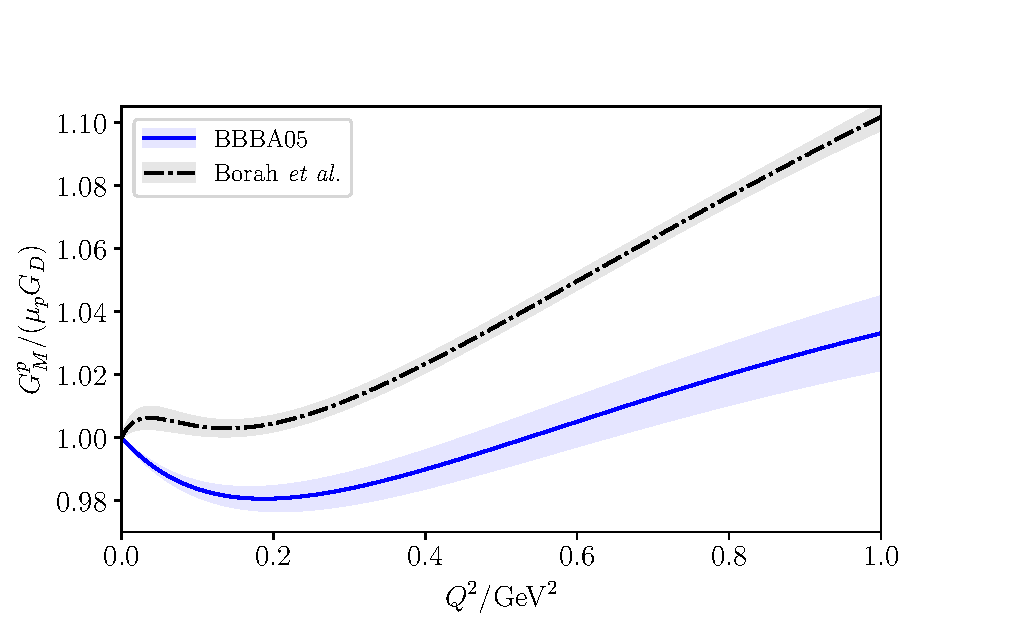
\includegraphics[width=0.7\textwidth]{plots/proton_magnetic-standalone.pdf}
 \vspace{4pt}
\caption{
Proton magnetic form factor normalized by a reference dipole ansatz
with a dipole mass of $0.84~{\rm GeV}$.
This plot is reproduced from Fig.~4 in Ref.~\cite{Borah:2020gte}
 and the associated supplemental data.
The proton-only fit to a $z$ expansion by Borah {\it et al.}~\cite{Borah:2020gte}
and the BBBA05 parameterization~\cite{Bradford:2006yz} are shown.
\label{fig:protonmagneticff}
}
\end{figure}
%------------------------------------------------------------------------------

However, there is a significant tension in existing parameterizations of the proton magnetic form factor extracted from that data, as
shown in Figure~\ref{fig:protonmagneticff}.
Two different parameterizations of the form factor, normalized by \del{the}\asm{a} dipole\asm{~parameterization},%
\begin{marginnote}
\entry{dipole parameterization}{$F_D(Q^2)\equiv (1+{Q^2}/{M_D^2})^{-2}$}
\end{marginnote}%
 are shown.%
\begin{marginnote}
\entry{BBBA05}{The Bradford, Bodek, Budd and Arrington 2005 nucleon elastic form factor parameterization~\cite{Bradford:2006yz}}
\end{marginnote}%
The BBBA05~\cite{Bradford:2006yz} are displayed as the lower (blue) band with a solid mean value.
A more recent $z$ expansion parameterization from Borah {\it et al.}~\cite{Borah:2020gte} is displayed by the upper (black) band with a dashed mean value.
The tension is significant over all $Q^2 > 0$, at the level of several percent,
including significant disagreement in the slope of the form factor at $Q^2 = 0$.
\del{Of the nucleon form factor calculations from LQCD,}%
\asm{LQCD computations of }the vector form factors are also the most mature \asm{of the nucleon matrix elements},
exhibiting no obvious tensions with experimental determinations
\sout{of the vector form factors }at their current level of precision.
A percent\asm{-}level calculation of the form factor $Q^2$ behavior \del{combined with}\asm{or} a direct calculation of the \del{slope of the }magnetic form factor \asm{slope could potentially }\del{would provide useful insight about this tension or could }discriminate
between the two parameterizations.

\sout{The nucleon axial form factor has had a much more complicated past than the vector form factors in LQCD.}%
\del{
\begin{marginnote}
 \entry{Axial \asm{vector coupling}\del{charge}} {The axial form factor at zero momentum transfer, $g_{\mathrm{A}} = F_{\mathrm{A}}(0)$}
\end{marginnote}%
}
The axial \del{charge}\asm{vector coupling}%
\footnote{Within the LQCD community, the axial vector coupling
 is commonly referred to as the axial charge.}%
\begin{marginnote}
 \entry{Axial \asm{vector coupling}\del{charge}} {The axial form factor at zero momentum transfer, $g_{\mathrm{A}} = F_{\mathrm{A}}(0)$}
\end{marginnote}%
 is a key benchmark for LQCD and is precisely known
from neutron decay experiments~\cite{Dubbers:2021wqv}.
LQCD calculations of the axial \del{charge}\asm{coupling} have historically been low compared to experiment~\cite{Aoki:2021kgd},
 and the discrepancy has been the topic of some controversy.
It is now understood that the treatment of excited state systematics is the main culprit for this discrepancy~\cite{Bar:2017kxh,Ottnad:2020qbw,Aoki:2021kgd}.
\asm{This topic, and how it pertains to the full momentum dependence of the form factor,
 will be discussed in detail in Sec.~\ref{sec:lqcd_pcac}.}
With proper control over the excited state contamination, LQCD calculations are now in good agreement with the experimental value~\cite{Jang:2019vkm,Gupta:2018qil,Alexandrou:2020okk,Abramczyk:2019fnf,Park:2021ypf,RQCD:2019jai,Hasan:2019noy,Djukanovic:2021yqg,Harris:2019bih,Liang:2018pis,Shintani:2018ozy,Ishikawa:2018rew}
 with one group achieving a sub-percent determination of $g_{\mathrm{A}}$~\cite{Chang:2018uxx,Berkowitz:2018gqe,Walker-Loud:2019cif}.

\sout{
 \textcolor{gray}{Armed with the newfound confidence in the control of systematics for the axial charge,}
 \textcolor{gray}{more emphasis is now being put into}}
\sout{
\asm{With more confidence in the ability to control the}
\asm{systematic errors for the axial vector coupling, LQCD collaborations now focus on computing}
 the \done{axial} form factor at nonzero momentum transfer \asm{in order}
 to make contact with the needs of the neutrino community and provide
 complementary constraints on free nucleon amplitudes.
}
{\textcolor{blue}{ {\bf [Wick's recommendation:]}
 \emph{The success in calculating the threshold value $g_A(0)$ motivates current efforts
 to map out $g_A(Q^2)$ of importance to the long-baseline neutrino program.}}}
\asm{The need for this is clear:} \done{sparse data from deuterium bubble-chamber experiments do not constrain
the axial form factor precisely.
The popular dipole ansatz has a shape that
is overconstrained by data resulting in an underestimated uncertainty.
Employing a model-independent $z$ expansion parameterization
relaxes the strict shape requirements of the dipole and yields
a more realistic uncertainty that is nearly an order of magnitude larger~\cite{Meyer:2016oeg}.
The axial radius, which is proportional to the slope of the form factor at $Q^2=0$,
has a 50\% uncertainty when estimated from the deuterium scattering data,
or $\approx35\%$ if deuterium scattering and muonic hydrogen are considered
together~\cite{Hill:2017wgb}.
Given that a modern $\nu N$ scattering experiment is extremely unlikely, LQCD is the only viable method to improve our understanding of the axial form factor to the required level of precision.
%Ideally, the lack of precision in the axial form factor would be rectified by a modern $\nu N$ scattering experiment.}
}

\done{Already,} one extremely striking feature of LQCD calculations \asm{of the axial form factor}
is the strong preference for a slower fall off \del{of the form factor }with increasing $Q^2$ than \asm{what is predicted by}\del{predicted by phenomenological determinations from} {\color{red} extractions from} experiment (\done{Section~\ref{sec:lqcd_results}}).
This preference is consistently reproduced by several lattice collaborations using
independent computation methods, lending more credence to the result.
\sout{When integrated over the full range of $Q^2$ to compute the nucleon cross section, this}
\asm{The nucleon cross section is obtained by integrating over $Q^2$, and the slower falloff with $Q^2$}
translates to an enhancement \sout{in the free nucleon cross section as large}
\asm{by as much} as 30--40\%
\del{over}\asm{for} neutrino energies greater than $1~{\rm GeV}$ (Section~\ref{sec:impact}).
In addition, the precision on the axial form factor uncertainty from LQCD
is small enough to be sensitive to the tension between vector form factor parameterizations.

The aforementioned situation with nucleon form factors is depicted in Figure~\ref{fig:nucleonxsec}.
The labels correspond to the following form factor parameterization choices and uncertainties:
\begin{description}
 \item[BBBA05] Vector form factors from BBBA05~\cite{Bradford:2006yz},
 and axial form factors from Meyer~{\it et al.}~\cite{Meyer:2016oeg}.
 The uncertainty is taken \asm{only} from \asm{the} BBBA05 \asm{parameterization},
 with all fit parameters assumed to be uncorrelated.
 \item[$z$ exp, vector] Vector form factors from Borah~{\it et al.}~\cite{Borah:2020gte},
 and axial form factors from Meyer~{\it et al.}~\cite{Meyer:2016oeg}.
 The uncertainty is taken \asm{only} from Borah~{\it et al.}
 \item[$z$ exp, ${\rm D}_{2}$ axial] \asm{the same} as ``$z$ exp, vector,''
 with the uncertainty taken \asm{only} from Meyer~{\it et al.} instead.
 \item[$z$ exp, LQCD axial] Vector form factors from Borah~{\it et al.}~\cite{Borah:2020gte},
 \asm{and the} axial form factor\del{s and their}\asm{~with its} uncertainty
 provided by authors from an LQCD simulation on a single physical mass ensemble.
\end{description}
Of particular note is the observed tension between the black and blue bands,
 which results from the tension between proton magnetic form factor parameterizations
 (see Figure~\ref{fig:protonmagneticff}).
The size of the \done{upper} red band with respect to the \done{lower, large} green band demonstrates the uncertainty reduction from replacing the deuterium scattering axial form factor with one obtained from LQCD. \del{and}The significant change in normalization is due to the slower fall off of the axial form factor.
Additionally, the size of the red band demonstrates the relevance of the tension in vector form factors, characterized by the difference between the black and blue curves, \change{with the uncertainty from LQCD a sub-dominant correction}\asm{{\bf [This is comparable, not subdominant?]}}.

%------------------------------------------------------------------------------
% nu-N cross section
\begin{figure}[hbt!]
 \centering
 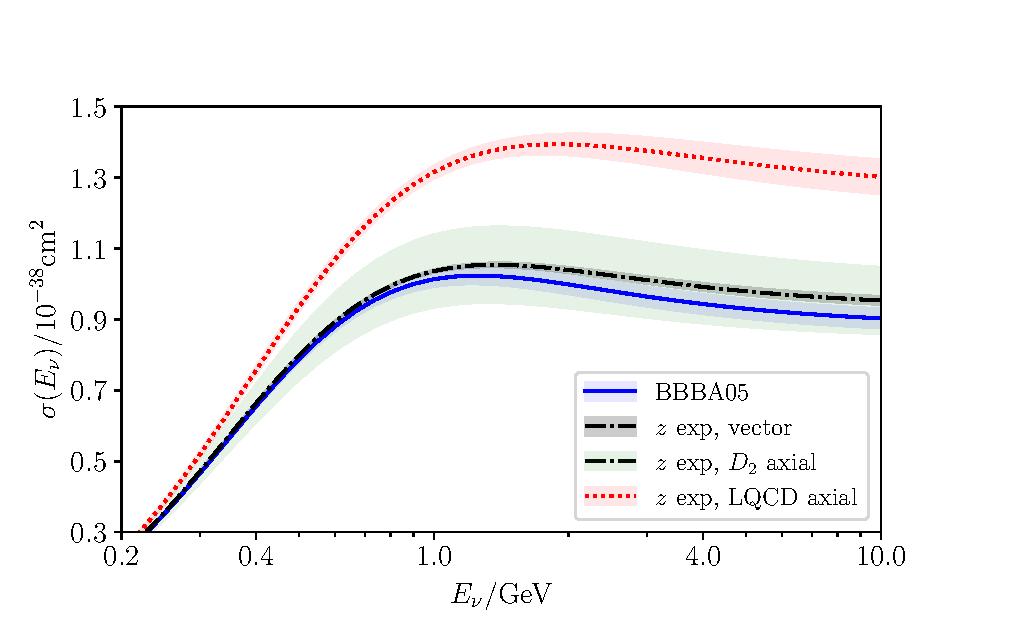
\includegraphics[width=0.7\textwidth]{plots/xsec_comparison-standalone.pdf}\vspace{4pt}
\caption{
 Neutrino cross sections on a free neutron, with their uncertainty bands,
 for various choices of parameterization explained in the bullet list provided in the \done{Section~\ref{sec:sof}}.
 \label{fig:nucleonxsec}
}
\end{figure}


% ------------------------------------------------------------------------------
% Lattice QCD
\section{LQCD determinations of the nucleon quasielastic form factor\label{sec:lqcd}}

LQCD has been and remains one of the major uses of the world's leadership computing facilities.
There is an extensive literature on LQCD covering the broad range of technical and formal aspects that are necessary to carry out state of the art calculations, for which we can not do justice in this review.
\del{Rather, f}For an in depth introduction to LQCD, we refer readers to the text books~\cite{Smit:2002ug,DeGrand:2006zz,Gattringer:2010zz}\del{ and i}\asm{. I}n this review, we provide a high-level summary of general issues that must be addressed as well as issues specific to LQCD calculations of nucleon matrix elements and form factors.
These issues are also discussed in detail in the bi-annual FLAG Reviews, see for example the most recent~\cite{Aoki:2021kgd}.%
%-------------------------------------------------------------------------------
\begin{marginnote}
\entry{FLAG}{Flavour Lattice Averaging Group}
\end{marginnote}


The promise of LQCD is to provide \change{Standard Model} predictions of low-energy hadronic and nuclear quantities with fully quantified theoretical uncertainties. \sout{rooted in the Standard Model.}
\sout{In order to deliver upon this promise, there are }
\change{To achieve this goal,} several sources of systematic uncertainty \sout{which} must be \change{assessed}.
\sout{For all LQCD calculations, t} These include extrapolations to the continuum and infinite volume limits as well as an extrapolation or interpolation to the physical quark mass limit.
\sout{For the continuum extrapolation, a} At least three values of the lattice spacing, $a$, of $\mathrm{O}(a\lesssim0.12\textrm{ fm})$ are required to ascertain if the leading discretization corrections are sufficient or not to describe the observed scaling violations (do all three results lie on a straight line or can one detect higher-order curvature?).
For the finite volume effects, a rule of thumb has been established from experience, that one requires calculations with $m_\pi L \gtrsim4$ (where $L$ is the spatial extent of the lattice volume) in order to keep these finite size corrections at the level of $\lesssim1-2\%$ and at least qualitatively described by the leading analytic formulae.%
\begin{marginnote}
    \entry{$\chi$PT}{Chiral Perturbation Theory: the low-energy effective field theory of QCD}
\end{marginnote}%
For the light-quark mass dependence, $\chi$PT may be able to guide the extrapolations.
However, for the nucleon, the convergence of $\chi$PT is not yet established, even at the physical pion mass with evidence of lack of convergence for the nucleon mass and $g_{\mathrm{A}}$~\cite{Chang:2018uxx,Walker-Loud:2019cif}.
As we will discuss more in Section~\ref{sec:calc_anatomy}, \sout{for properties of nucleons, }there are two additional significant sources of \sout{systematic }uncertainty \asm{for nucleons }which are the exponentially%
\begin{marginnote}
    \entry{S/N}{Signal-to-noise}
\end{marginnote}%
degrading S/N problem \del{for nucleons }and excited state contamination.



%-------------------------------------------------------------------------------
% LQCD Intro
\subsection{LQCD: a high level summary}
The QCD path integral is quadratic in the quark fields allowing for an analytic integration over the fermionic fields\del{ such that i}\asm{. I}n Euclidean space, one has the gluonic integral
\begin{equation}\label{eq:Z_QCD}
Z_{\mathrm{QCD}} = \int D U\, {\rm Det}[\Dslash(U) + m_q]\, e^{-S_{\mathrm{G}}(U)},
\end{equation}
with gluon action $S_{\mathrm{G}}(U)$ and the determinant of the quark operator ${\rm Det}[\Dslash(U) + m_q]$, for each flavor of quark simulated.
Even at finite lattice spacing and volume, the multi-dimensional integral is vastly too large to perform.
However, in Euclidean space, \asm{both $S_{\mathrm{G}}$ and }the fermion determinant \del{is}\asm{are} real and positive for zero chemical potential, \sout{as well as $S_{\mathrm{G}}$, }and so the integral can be approximated with an HMC algorithm~\cite{Duane:1987de} using the factor ${\rm Det}[\Dslash(U) + m_q]\, e^{-S_{\mathrm{G}}(U)}$ as the importance sampling weight.%
%-------------------------------------------------------------------------------
\begin{marginnote}
\entry{HMC}{Hybrid Monte Carlo}
\entry{Configurations}{Samples of the gluon field}
\entry{Ensemble}{A set of configurations all generated with the same bare QCD parameters}
\end{marginnote}%
%-------------------------------------------------------------------------------
In this way, a large number of configurations of gauge fields can be generated, providing \done{a stochastic determination of the} \sout{estimates of} correlation functions
\begin{equation}
\langle O \rangle = \frac{1}{N_{\rm cfg}}\sum_{i=1}^{N_{\rm cfg}} O[U_i]
    +\mathrm{O}\left(\frac{1}{\sqrt{N_{\rm cfg}}} \right)\, ,
\end{equation}
where $O[U_i]$ is the correlation function evaluated on configuration $i$.
The most expensive part of generating the configurations is evaluating the fermion determinant for the light and strange quarks.
This is done with the use of pseudo-fermions (bosonic fields, $\phi$)
\begin{equation}
Z_\psi = \int D\bar{\psi}D\psi\, e^{-\bar{\psi}[\Dslashe[U]+m_q]\psi}
    = {\rm Det}[\Dslash(U) + m_q]
    = \int D\phi^\dagger D\phi\, e^{-\phi^\dagger \frac{1}{\Dslashe[U]+m_q} \phi}
\end{equation}
for which the bilinear operator is the inverse of the Dirac operator, which is a large, sparse matrix.
Most of the algorithmic development for accelerating LQCD has gone into efficiently solving these large sparse matrices with large condition numbers.  In particular, this is a problem very well suited for GPUs
for which we have an advanced library, QUDA~\cite{Clark:2009wm,Babich:2011np}, developed for the international community.%
%-------------------------------------------------------------------------------
\begin{marginnote}
\entry{GPU}{Graphical Processing Unit}
\end{marginnote}%
%-------------------------------------------------------------------------------


There are many valid choices one can make in constructing the discretized lattice action, provided continuum QCD is recovered as $a\rightarrow0$.
This is known as the universality of the continuum limit, with each choice only varying at finite lattice spacing.
Deviations from QCD, which arise at finite $a$, are often called \textit{discretization corrections} or \textit{scaling violations}.%
%-------------------------------------------------------------------------------
\begin{marginnote}
\entry{Universality}{All valid choices of discretized QCD become QCD as $a\rightarrow0$}
\entry{EFT}{Effective field theory}
\end{marginnote}%
%-------------------------------------------------------------------------------
\sout{That all lattice actions reduce to QCD as $a\rightarrow0$ is known as the universality of the continuum limit.  It}
\done{Universality} is a property \asm{that}\del{which} can be proved in perturbation theory but must be established numerically given the non-perturbative nature of QCD.  For sufficiently small lattice spacings, one can use EFT to construct a continuum theory that encodes the discretization effects in a tower of higher dimensional operators. This is known as the Symanzik EFT for lattice actions~\cite{Symanzik:1983dc,Symanzik:1983gh}.
One interesting example involves the violation of Lorentz symmetry at finite lattice spacing: in the Symanzik EFT, the operators \asm{that}\del{which} encode \sout{this }Lorentz violation scale as $a^2$ with respect to the operators \asm{that}\del{which} survive the continuum limit\del{, and t}\asm{. T}hus, Lorentz symmetry is an accidental symmetry of the continuum limit.  It is not respected at any finite lattice spacing, but the measurable consequences vanish as $a^2$ for sufficiently small lattice spacing.

\change{As a concrete} 
example\asm{~of the Symanzik EFT}, consider the discretized gluon action.
The link fields are Wilson lines
\begin{equation}
U_\mu(x) = \exp\left\{i a\int_0^1 dt A_\mu(x +(1-t)a\hat{\mu}) \right\}
    \approx \exp\left\{i a \bar{A}_\mu(x) \right\}\, .
\end{equation}
The gluon field $A_\mu(x)$ can be approximated as constant over the interval $[x, x+a\hat{\mu}]$, as expressed by $\bar{A}_\mu(x)$, with $a$ being the lattice spacing.
This parameterization allows for the construction of a discretized theory \asm{that}\del{which} preserves gauge-invariance~\cite{Wilson:1974sk}, a key property of gauge theories.
In the continuum, the gluon action-density is given by the product of field strength tensors, which are gauge-covariant curls of the gauge potential.
When constructing the discretized gluon-action, it is therefore natural to use objects which encode this curl of the gauge potential.  The simplest such object is referred to as a ``plaquette'' and given by
\begin{equation}
\hspace{-1.25in}\Umunu \hspace{-0.65in}
    =U_{\mu\nu}(x)
    =U_\mu(x)U_\nu(x+a\hat{\mu}) U^\dagger_\mu(x+a\hat{\nu}) U^\dagger_\nu(x)\, .
\end{equation}
For small lattice spacing, this Wilson gauge-action reduces to the continuum action plus irrelevant (higher dimensional) operators which vanish in the continuum limit
\begin{align}\label{eq:gluon_action}
S_{\mathrm{G}}(U) &= \beta \sum_{n=x/a} \sum_{\mu<\nu}
    \textrm{Re}\left[ 1 - \frac{1}{N_c} \textrm{Tr} \left[U_{\mu\nu}(n) \right]\right]
\nonumber\\&=
    \frac{\beta}{2N_c}
    a^4 \sum_{n=x/a,\mu,\nu}
    \left[
        \frac{1}{2} \textrm{Tr} \left[ G_{\mu\nu}(n)G_{\mu\nu}(n)\right]
        +\mathrm{O}(a^2)
    \right]\, ,
    & \rightarrow \beta = \frac{2N_c}{g^2}\, .
\end{align}
The continuum limit, which is the asymptotically large $Q^2$ region, is therefore approached as $\beta\rightarrow\infty$ where $g(Q^2)\rightarrow 0$.%
\begin{marginnote}
\entry{Irrelevant operators}{In the renormalization sense, these are operators of mass dimension $[O]>4$, such that their dimensionfull couplings scale as $a^n=\Lambda^{-n}$ where $\Lambda$ is a high energy scale
that goes to infinite in the continuum limit for LQCD, and $n=[O]-4$}
\end{marginnote}


The inclusion of quark fields adds more variety of lattice actions, each with their own benefits and drawbacks.
There are four commonly used fermion discretization schemes which are known as staggered fermions~\cite{Kogut:1974ag,Banks:1975gq,Banks:1976ia,Susskind:1976jm}, clover-Wilson fermions~\cite{Sheikholeslami:1985ij}, twisted mass fermions~\cite{Frezzotti:2000nk} and DWF~\cite{Kaplan:1992bt,Shamir:1993zy,Furman:1994ky}.%
%-------------------------------------------------------------------------------
\begin{marginnote}
\entry{DWF}{Domain Wall Fermions}
\end{marginnote}%
%-------------------------------------------------------------------------------
In this review, we comment that:
\begin{itemize}[leftmargin=*]
\item Staggered fermions are the least expensive \del{numerically }to simulate\asm{~numerically}, have leading scaling violations of $\mathrm{O}(a^2)$, and they have a remnant chiral symmetry protecting the quark mass from additive mass renormalization.  However, they split the four components of the fermion spinor onto different components of a local hypercube, mixing the Dirac algebra with spacetime translations.  This significantly complicates their use for baryons~\cite{Golterman:1984dn,Bailey:2006zn,Lin:2019pia}.

\item Clover-Wilson fermions are the most commonly used discretization scheme given their theoretical simplicity and preservation of all symmetries except chiral symmetry.  The explicit breaking of chiral symmetry with the Wilson operator means the light quark masses must be finely tuned against ultra\del{-}violet chiral symmetry breaking that scales as $1/a$, after which there remain residual $\mathrm{O}(a)$ chiral symmetry breaking effects.  It is well known, albeit laborious, how to non-perturbatively remove these leading $\mathrm{O}(a)$ scaling violations~\cite{Luscher:1996sc,Luscher:1996ug,Luscher:1996jn,Capitani:1998mq}, which must be done for both the action as well as matrix elements.

\item Twisted mass fermions are a variant of Wilson fermions that exploits the approximate $SU(2)$ chiral symmetry of QCD to introduce a twisted quark mass term, $i\mu\g_5 \tau_3$.  At \asm{maximal twist}, the bare quark mass is cancelled by the $1/a$ additive quark mass, leaving $\mu$ as the only contribution through $\mathrm{O}(a)$ to the physical quark mass.  All observables are automatically \asm{$\mathrm{O}(a)$ improved} at maximal twist~\cite{Frezzotti:2003ni}.
\asm{\bf [``maximal twist'', ``$\mathrm{O}(a)$ improved'' are both jargon]}
However, twisted mass fermions break isospin symmetry at finite lattice spacing, \del{causing}\asm{which causes} some complications now that LQCD results are precise enough to \sout{require}\asm{resolve} isospin breaking corrections from $m_d-m_u$ and%
\begin{marginnote}
\entry{QED}{Quantum electro-dynamics}
\end{marginnote}%
QED\sout{ to be compared with experiment}.

\item The fourth most common discretization are DWF, which introduce a fifth dimension to the theory with unit links (the gluons are not dynamic in the fifth dimension) with the left and right handed fermions bound to opposite sides of the fifth dimension of size $L_5$.  The overlap of these left and right modes gives rise to an explicit chiral symmetry breaking that is exponentially suppressed by the extent of the fifth dimension.  For sufficiently small chiral symmetry breaking (large $L_5$), DWF are also automatically \asm{$\mathrm{O}(a)$ improved}.
While very desirable, DWF are \del{numerically }more expensive to simulate\asm{~numerically}, both because of the extra fifth dimension and also because the algorithmic speed up offered by multi-grid\asm{~computational technique}, which works tremendously for clover-Wilson fermions on GPUs~\cite{Clark:2016rdz}\del{,} \done{but} is not yet \asm{fleshed}\del{flushed} out for DWF~\cite{Boyle:2014rwa,Cohen:2011ivh,Yamaguchi:2016kop,Brower:2020xmc,Boyle:2021wcf}.

\item A final common variant of action is one in which the fermion discretization used in the generation of the gauge fields (the sea quarks) and the action used when generating quark propagators (the valence quarks) are different: this is known as a \textit{mixed action}~\cite{Renner:2004ck}.
The most common reason to use such an action is to take advantage of numerically less expensive methods to generate the configurations while retaining good chiral symmetry properties of the valence quarks, which is known to suppress chiral symmetry breaking effects from the sea-quarks~\cite{Bar:2002nr,Bar:2005tu,Tiburzi:2005is,Chen:2007ug}.

\end{itemize}
As mentioned above, a key assumption of LQCD is that all varieties of lattice action, for sufficiently small lattice spacing, are approximated by continuum QCD plus irrelevant operators whose contributions vanish in the continuum limit.
It is important for the field to test this assumption of universality by computing the same quantities with a variety of lattice actions, both at the level of gluons as well as the fermions, in order to gain confidence in the results that are extrapolated to the physical point.


% ------------------------------------------------------------------------------
% anatomy of LQCD calculation
\subsection{Anatomy of LQCD calculations of nucleon form factors\label{sec:calc_anatomy}}

In order to determine the mass of the nucleon (or any hadron), we rely on the construction of two-point correlation functions that are constructed in a mixed time-momentum representation, most commonly utilizing spatially local creation operators (sources) and momentum space annihilation operators (sinks).
The non-perturbative nature of QCD means we do not know how to construct the nucleon wave function, and so we utilize \textit{interpolating operators} which have the quantum numbers of the state we are interested in.
These creation and annihilation operators will couple to all eigenstates of QCD with the same quantum numbers giving rise to a two-point function with a spectral decomposition
\begin{align}\label{eq:2pt}
    C(t,\mathbf{p}) &= \sum_{\mathbf{x}} e^{-i \mathbf{p\dotp x}}
        \langle \O| O(t,\mathbf{x}) O^\dagger(0,\mathbf{0}) | \O \rangle
%\nonumber\\&=
    =
    \sum_{n=0}^\infty z_n(\mathbf{p}) z_n^\dagger(\mathbf{p}) e^{-E_n(\mathbf{p})t}\, .
\end{align}
In this expression, $|\O\rangle$ is the vacuum state,
$z_n(\mathbf{p}) = \sum_{\mathbf{x}}e^{-i\mathbf{p\dotp x}} \langle \O|O(0,\mathbf{x})|n\rangle$
and $z_n^\dagger(\mathbf{p}) = \langle n(\mathbf{p})|O^\dagger(0,\mathbf{0})|\O\rangle$.
To go from the first equality to the second, we have inserted a complete set of states, $1=\sum_n |n\rangle\langle n|$ and we have used the time-evolution operator to shift the annihilation operator to $t=0$ and expose the explicit time dependence.%
%-------------------------------------------------------------------------------
\begin{marginnote}
\entry{$O(t,\mathbf{x}) = e^{\hat{H}t} O(0,\mathbf{x}) e^{-\hat{H}t}$}{The Hamiltonian, $\hat{H}$, is used to time evolve the operator}
\end{marginnote}%
%-------------------------------------------------------------------------------
Momentum conservation selects only the state $n(\mathbf{p})$ in the sum over all states enabling the use of this mixed spatial creation operator and momentum annihilation operator.
As we will discuss in more detail below, it is more desirable to instead creation operators
in momentum space rather than position space.
They are not commonly used as they are significantly more expensive numerically to generate.

For large Euclidean time, the correlation function will be dominated by the ground state as the excited states will be exponentially suppressed by the energy gap
\begin{equation}
    C(t) = z_0 z_0^\dagger e^{-E_0 t}\left[
        1 + r_1 r^\dagger_1 e^{-\Delta_{1,0}t} + \cdots \right]\, .
\end{equation}%
\begin{marginnote}
\entry{$\D_{m,n}= E_m - E_n$}{energy gap}
\entry{$r_n = z_n / z_0$}{ratio of overlap factors}
\end{marginnote}%
It is useful to construct an \textit{effective mass} to visualize at which time $t$, the ground state begins to saturate the correlation function
\begin{align}
m_{\rm eff}(t) &= \ln \left( \frac{C(t)}{C(t+1)} \right)
%\nonumber\\&=
    =
    E_0 + \ln\left( 1 + \sum_{n=1} r_n r^\dagger_n e^{-\Delta_{n,0}t}\right)\, .
\end{align}


A well known challenge which complicates the analysis is that for nucleon two-point functions, the S/N ratio degrades exponentially at large Euclidean time~\cite{Lepage:1989hd}
\begin{equation}
\lim_{{\rm large}\ t} {\rm S/N}%\frac{\mathrm{Signal}}{\mathrm{Noise}}
    \propto \sqrt{N_{\mathrm{sample}}} e^{-(m_{\mathrm{N}} - \frac{3}{2}m_\pi)t}\, ,
\end{equation}
which adds an extra source of excited state systematic uncertainty that must be quantified.
\change{In} the region in time when the ground state begins to saturate the correlation functions, at $t\approx 1$~fm, the noise \change{becomes} significant, making the correlation functions in this region susceptible to correlated fluctuations which can bias a simplistic single-state analysis.
Further, as the pion mass is reduced towards its physical value, the excited state energy gap also shrinks, as the lowest lying excited state is typically a nucleon-pion in a relative $P$-wave.  At the same time, the energy scale which governs the exponential degradation of the signal also grows.  The former issue means calculations must be performed at larger Euclidean time to suppress the smaller gapped excited states and the latter issue means we need exponentially more statistics to obtain a fixed relative uncertainty at a given time.
In order to boost statistics, given the numerical cost of generating more configurations, time and spatial translation invariance are used to generate sources at several choices of $t_0$ and $\mathbf{x}_0$, which are then translated back to the origin and averaged together.  For the nucleon, it was observed that hundreds of sources on each configuration, using an anisotropic clover-Wilson ensemble~\cite{HadronSpectrum:2008xlg}, still showed approximate $\sqrt{N_{\rm sample}}$ improvement of the stochastic uncertainty as a function of the number of sources per configuration~\cite{Beane:2009kya}.



The most common method of constructing three-point correlation functions follows a similar strategy, beginning with spatially local sources.
A nucleon three-point function with current $j_\G$ is constructed with interpolating operators $N(\tsep,\mathbf{x})$ and $N^\dagger(0,\mathbf{0})$,
\begin{align}
C_\G(\tsep,\t) &= \sum_{\mathbf{x,y}}e^{-i\mathbf{p\dotp x} +i\mathbf{q\dotp y}}
    \langle\O|N(\tsep,\mathbf{x}) j_\G(\t,\mathbf{y}) N^\dagger(0,\mathbf{0}) |\O\rangle
\nonumber\\&=
    \sum_{n,m} z_n(\mathbf{p})z_m^\dagger(\mathbf{p-q})e^{-E_n(\tsep-\t)}e^{-E_m \t} g_{n,m}^\G\, ,
\end{align}
where $g_{n,m}^\G$ are the matrix elements of interest, and in principle, all other quantities can be determined from the two-point function, a point we will return to.
Often, the sink is projected to zero momentum, $\mathbf{p}_n=0$, for which momentum conservation gives the momentum of the incoming state to be $\mathbf{p}_m = -\mathbf{q}$.%
%-------------------------------------------------------------------------------
\begin{marginnote}
\entry{$j_\G = \bar{q}\, \G\, q$}{quark bilinear currents of Dirac structure $\G$ and unspecified flavor structure}
\entry{$g_{n,m}^\G = \langle n| j_\G |m\rangle$}{hadronic matrix elements of interest from state $m$ to $n$ with implicit momentum and energy dependence}
\entry{$\tsep$}{The time-separation between the sink and source}
\end{marginnote}%
%-------------------------------------------------------------------------------
A typical calculation is performed with a sequential propagator~\cite{Martinelli:1988rr}
whose source is constructed by taking the forward propagators from the origin and contracting all but one spin and color index at the sink time, $\tsep$.%
% FOOTNOTE ---------------------------------------------------------------------
\footnote{There are alternative methods for computing nucleon structure known as the one-end trick~\cite{Foster:1998vw,McNeile:2006bz,Alexandrou:2013xon} and a variant of the Feynman-Hellmann Theorem~\cite{CSSM:2014uyt}, but these are not in wide use.}
%-------------------------------------------------------------------------------

Each choice of $\tsep$, flavor and spin of the initial and final state, and each choice of flavor for the current requires a new sequential propagator, rendering this aspect of the computation relatively expensive.
While each sequential propagator can only be used for these specific choices, one is free to insert any quark bilinear operator for the current, including non-trivial spatial structure and momentum.
To boost statistics, in addition to taking advantage of translation invariance as with the two-point function, the \textit{coherent sink technique}~\cite{LHPC:2010jcs} is used to solve a single sequential propagator for many choices of the origin.

The most significant challenge in determining the nucleon matrix elements and subsequent form factors is dealing with the excited state contamination, an issue that is compounded by the degrading S/N.
If the nucleon two-point function is becoming saturated by the ground state at $t\approx1$~fm, the ideal three-point function would use values of $\tsep\approx2$~fm.
In practice, a few values of $\tsep$ in the range $0.8 \lesssim \tsep \lesssim 1.5$~fm are used because the S/N ratio of the three-point functions decays more rapidly than the two-point function, and an extrapolation to large $\tsep$ is used to isolate the ground state matrix elements.
However, using just one excited state in the analysis requires three values of $\tsep$ to have a one degree-of-freedom fit to extract the ground state matrix element.
Most results have been generated with three or fewer values of $\tsep$.
Ref.~\cite{Chang:2018uxx} utilized many values of $\tsep$ to determine $g_{\mathrm{A}}$, \change{and} a few \change{other} groups have begun advocating for the use of many values of $\tsep$, including small values, to improve our ability to understand and control the excited state contamination~\cite{Hasan:2019noy,Alexandrou:2019brg,He:2021yvm}.
Ref.~\cite{He:2021yvm} utilized 13 values of $\tsep$, which allows for a systematic study of the uncertainty associated with truncating early and/or late values of $\tsep$ in the analysis, as well as providing sufficient data to perform up to a complete 5-state fit.

At non-zero momentum, the excited states become more problematic.  While the energy associated with the signal grows with the momentum, the energy scale associated with the noise is independent of the momentum and thus their difference, which is the energy scale that governs the decay of the S/N, grows with increasing momentum.
For values of $Q\gtrsim 2$~GeV, the noise becomes unmanagable unless one uses a smearing profile that couples more strongly to boosted nucleons~\cite{Bali:2016lva}.
For boosted nucleons, parity is also no longer a good quantum number and so the correlation function begins to mix even and odd parity states through the matrix elements.  Such contamination can be handled through a variational method that incoporates even and odd parity nucleons~\cite{Stokes:2013fgw,Stokes:2018emx,Stokes:2019zdd}.



Recent results have uncovered some additional aspects of excited state contamination:
\begin{itemize}[leftmargin=*]
\item Two-point functions constructed as in Equation~\eqref{eq:2pt} are insufficient to reliably determine any of the excited states.  Different choices of $\tmin$ and different reasonable priors in a Bayesian analysis support excited states that differ by several sigma, also resulting in sensitivity of the ground state spectrum~\cite{Park:2021ypf,He:2021yvm} and matrix elements~\cite{Jang:2019vkm,Gupta:2021ahb}.

\item In contrast, the curvature in the three-point functions associated with the current insertion time \change{provides extra constraints that make the determination of the spectrum stable and robust}
\del{is very constraining on the excited state spectrum, resulting in very stable and robust determination of the spectrum}
while varying $\tmin$, the number of excited states, the excited state model and the excited state priors~\cite{He:2021yvm}.
While it is encouraging that the spectrum and matrix elements become very stable, such an analysis offers no insight into the nature of the excited states.  For example, with typical values of $m_\pi L\approx4$, the $P$-wave $N(\mathbf{p})\pi(-\mathbf{p})$ excited state energy gap is essentially the same as the $N\pi\pi$ threshold state.%
\begin{marginnote}
 \entry{$N\pi$}{Nucleon-pion}
 \entry{$N\pi\pi$}{Nucleon and two pion}
\end{marginnote}

\item Many groups determine the spectrum and overlap factors from fits to the two-point functions, and then pass these results into the three-point function analysis without allowing the values to adjust to the global minimum.  Such a choice can either lead to an overestimate of the uncertainty of the three-point functions (if one uses the variability of the spectrum mentioned above), or a biased extraction of the ground state matrix elements (if one uses the ``wrong'' value of the spectrum).  Given the computational setup described above, the robust choice is to perform a global analysis of the two- and three-point functions simultaneously.

\item For zero-momentum transfer, where the spectrum of the in and the out states have the same value,
the use of the summation method~\cite{Maiani:1987by} or a variant of the Feynman-Hellman method~\cite{deDivitiis:2012vs,Bouchard:2016heu}, \del{which is closely related to the summation method,} it is understood that the excited states become significantly suppressed compared to the three-point function~\cite{Capitani:2012gj,He:2021yvm}.
For non-zero momentum transfer, 
\change{only the Breit-Frame where the momentum of the in and out states is equal and opposite, is amenable to this alternative method~\cite{Gambhir:2019pvw}.}
\del{such a technique can only be used well in the Breit-Frame where the momentum of the in and out states is equal and opposite, such that the energy spectrum is the same~\cite{Gambhir:2019pvw}.}

\item The excited state contamination is particularly relevant for the PCAC relation, which we discuss in more detail in Section~\ref{sec:lqcd_pcac}.


\end{itemize}


% ------------------------------------------------------------------------------
% LQCD PCAC
\subsection{Role of PCAC in LQCD results of $F_{\mathrm{A}}(Q^2)$\label{sec:lqcd_pcac}}

$F_{\rm A}(Q^2)$ can be isolated in LQCD calculations with particular kinematic choices that are not contaminated by the induced pseudoscalar form factor, see for example Ref.~\cite{Gupta:2017dwj}.
Given the challenges in identifying all the sources of systematic uncertainty in the calculation of $g_{\mathrm{A}}$, particularly the excited state contamination, it is prudent to perform cross checks of observables to test for consistency of the results.
The validity of the PCAC relation,
\begin{align}
 \partial^\mu A^{a}_{\mu}(x) = 2 m_q P^{a}(x),
 \label{eq:pcac}
\end{align}
provides a complex consistency check.
Here, $A^{a}_\mu$ and $P^{a}$ are the axial and pseudoscalar currents,
 respectively, and $m_q$ is the light quark mass.
The PCAC relation is an exact symmetry in the continuum limit.
The generalization of this relation to the nucleon form factors
 yields the GGT%
 \begin{marginnote}
 \entry{GGT}{Generalized Goldberger-Triemann relation (Equation~\eqref{eq:ggt})}
 \end{marginnote}%
 relation,
\begin{align}
 2 m_{\mathrm{N}} F_{\mathrm{A}}(Q^2) -\frac{Q^2}{2m_{\mathrm{N}}} \widetilde{F}_{\mathrm{P}}(Q^2) = 2 m_q F_{\mathrm{P}}(Q^2),
 \label{eq:ggt}
\end{align}
 which provides orthogonal checks of individual matrix elements
 for the axial and pseudoscalar currents.
The axial, induced pseudoscalar, and pseudoscalar form factors of the nucleon
 ($F_{\mathrm{A}}$, $\widetilde{F}_{\mathrm{P}}$, and $F_{\mathrm{P}}$, respectively) appear in this expression,
 and $m_{\mathrm{N}}$ is the nucleon mass.
The PPD ansatz, which is only approximate even in the continuum limit,% is also studied,%
\begin{marginnote}
 \entry{PPD}{Pion pole dominance}
 \end{marginnote}%
\begin{align}
 \widetilde{F}^{\rm PPD}_{\mathrm{P}}(Q^2) = \frac{4m_{\mathrm{N}}^2}{Q^2+m_\pi^2} F_{\mathrm{A}}(Q^2),
 \label{eq:ppd}
\end{align}
is obtained
 by carefully considering the leading asymptotic behavior of the
 form factors in the double limit $Q^2\to0$ and $m_q\to0$~\cite{Sasaki:2007gw}.

Initial calculations targeting the axial form factor verified the PCAC relation
 for the full correlation functions but found significant \emph{apparent} violations
 of GGT~\cite{Ishikawa:2018rew,Gupta:2017dwj,Bali:2018qus}. The resolution of this apparent violation
 is now informed by baryon $\chi$PT, which suggests that chiral
 and excited state corrections to the spatial axial, temporal axial, and induced pseudoscalar
 are functionally different and not properly removed.
The axial contributions are largely dominated by loop-level $N\pi$ excited states
 with a highly suppressed tree-level correction.
The correction to the axial current is nearly independent of $Q^2$.
On the other hand, corrections to the induced pseudoscalar are
 driven by the tree-level correction and has
 a strong $Q^2$ dependence~\cite{Bar:2018xyi}, with the largest correction at low $Q^2$.
The $N\pi$ loop contribution in the induced pseudoscalar is highly suppressed by
 an approximate cancellation.
The contamination to the pseudoscalar current is redundant with the
 axial and induced pseudoscalar chiral corrections and can be obtained
 by application of the PCAC relation.

Scrutiny of the LQCD data has demonstrated many of the features
 that were expected from chiral perturbation theory.
$N\pi$ states were initially expected to be negligible due to a volume suppression
 of the state overlap, which makes them invisible to the two-point functions~\cite{Bar:2016uoj}.
However, the three-point axial matrix element can enhance these contributions relative
 to the ground state nucleon matrix element, which is enough to overcome the volume suppression.
The primary excited state contaminations to the temporal axial form factor matrix elements
 were shown to be driven by two specific $N\pi$ states,
 characterized by a transition through an axial current
 of the nucleon state to an $N\pi$ excited state or vice versa~\cite{Jang:2019vkm}.
In the language of $\chi$PT, these states contribute to tree-level nucleon-pion graphs with fixed relative momentum~\cite{Bar:2018xyi}.
In contrast to the temporal axial insertion, the spatial axial insertion
 is instead expected to be more strongly affected by a tower of loop-level
 $N\pi$ corrections~\cite{Bar:2018xyi}.
Taking into account these observations,
 analyses that fix the spectrum using the two-point functions alone
 will often miss the important $N\pi$ contamination to the
 axial matrix element~\cite{Jang:2019vkm,He:2021yvm}.


Nucleon matrix elements of the temporal axial current have the largest visible excited state contamination~\cite{Jang:2019vkm,RQCD:2019jai} which can be at least qualitatively understood with $\chi$PT~\cite{Bar:2018xyi}.
This has led to new analysis strategies that more carefully deal with the $N\pi$ excited state with pion-pole contributions, yielding minimal violations of PCAC that include such matrix elements, as well as improved understanding of excited state contamination on matrix elements sensitive to $F_{\rm A}(Q^2)$ or $\tilde{F}_{\rm P}(Q^2)$, which previously exhibited deviations as large as $40\%$ from the PPD or GGT
 ansatz at low $Q^2$, where it was expected to
 work best~\cite{Bali:2014nma,Gupta:2017dwj}.


\del{\textcolor{gray}{ While these results are very encouraging, they are not conclusive in the sense that they require us to impose our theoretical prior on the analysis, rather than the results naturally ``falling out'' from the numerical analysis.
}}
\asm{These results are very encouraging,
 but must be reproduced by several independent LQCD calculations for validation.
At the time of writing,
 not all of the results are free from imposed theoretical expectations.}
In order to achieve \del{this}\asm{a} more stringent validation, the calculations would have to generally be performed \del{at larger source-sink separation times }where the correlation functions are \del{all }saturated by the ground state\asm{.
This could be accomplished by taking the correlation function at large Euclidean times},
 but the noise is exponentially larger.
Given the extreme cost of \asm{using }such a strategy, a better \del{solution }\asm{alternative }would be to implement a variational method that allows for the use of multi-hadron operators that can explicitly remove the $N\pi$ excited states through a diagonalization of the correlation functions~\cite{Blossier:2009kd}.  We will return to this point in Section~\ref{sec:future}.


% ------------------------------------------------------------------------------
% LQCD results
\subsection{Survey of LQCD results of $F_{\mathrm{A}}(Q^2)$\label{sec:lqcd_results}}

The main deliverables from LQCD calculations of the axial form factor
 are the axial and induced pseudoscalar form factors taken in the continuum,
 infinite volume and physical pion mass limits, complete with a set of parameterization coefficients
 and covariance matrix.
Though the axial \asm{vector coupling}
 and \asm{axial }radius are useful for connecting with low-energy applications,
 such as pion electroproduction and neutron decay,
 the needs of neutrino physics in the few-GeV energy range depend
 on the full momentum transfer dependence of the form factor.
 This is especially true considering the agreement between LQCD and experiment
 for the axial radius taken together with the observation that
 LQCD prefers a slower form factor fall off than experiment,
 as shown in Figure~\ref{fig:gaq2_overlay}.
If the axial radius were the only parameter determining the form factor $Q^2$ dependence,
 then these two observations are incompatible.
Though the form factor shape, especially when allowed to explore its full uncertainty,
 is decidedly \emph{not} a dipole, the central value curve determined
 from experiment appears to be dipole-like.
Restricting to dipole shape only, agreement with the axial radius at $Q^2=0$
 would mean the axial form factor should agree over the entire relevant $Q^2$ range,
 a statement that is not supported by the LQCD data.
There is no reason to expect nature to prefer a dipole-like parameterization ---
 the experimental preference toward a dipole-like parameterization is based on
 a few datasets from the 1970's and 1980's~\cite{ANL_Barish_1977, BNL_Baker_1981, Kitagaki:1983px}
 with $O(10^3)$ events at most,
 on deuterium targets with nuclear corrections that are likely underestimated~\cite{Meyer:2016oeg}.
In addition, the dipole parameterization violates
 unitarity constraints imposed by QCD~\cite{Bhattacharya:2011ah},
 and although it has the expected asymptotic behavior at high-$Q^2$,
 this occurs for a regime well outside of the kinematic range probed
 by neutrino scattering experiments.



Figure~\ref{fig:gaq2_overlay} shows the status of existing calculations of
 the nucleon axial form factor from LQCD,
 compared to the axial form factor obtained from neutrino scattering
 with deuterium in Ref.~\cite{Meyer:2016oeg}.
The RQCD~\cite{RQCD:2019jai} and NME~\cite{Park:2021ypf} collaborations
 have the most mature analyses with several ensembles that probe a range of
 systematic effects.
These computations each have their own methods for addressing the
 excited state contaminations discussed in Section~\ref{sec:lqcd_pcac},
 which successfully restore the GGT relation.
RQCD modify the parameterization used to fit the correlation function
 to better constrain the expected shape of excited state contamination from the $N\pi$ states based upon expectations from $\chi$PT~\cite{Bar:2018xyi}.
NME test a variety of Bayesian fits to constrain the excited state contributions,
 where their preferred fit enforces a tight prior on the nucleon-pion state
 at the energy expected from a naive dispersion relation.
Because these two results are based on several ensembles,
 their fits are parameterized and plotted as bands rather than as scatter points
 to distinguish them from estimates on single ensembles.

\begin{figure}[hbt!]
\centering
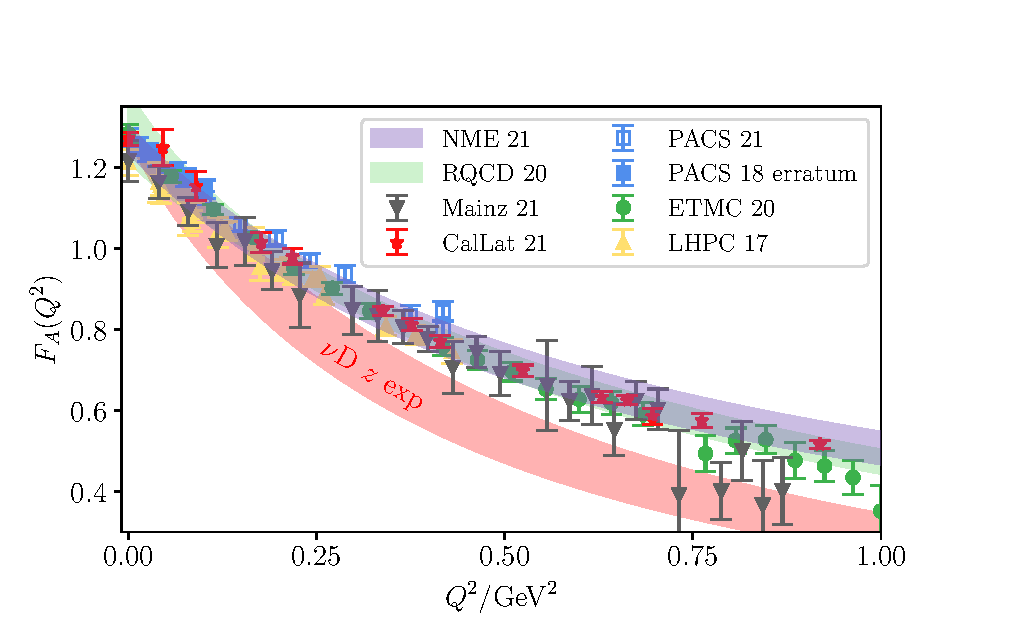
\includegraphics[width=0.75\textwidth]{plots/gaq2-overlay-standalone.pdf}
\vspace{10pt}
\caption{
Published results for the axial form factor obtained from LQCD,
 compared with the deuterium extraction from Ref.~\cite{Meyer:2016oeg}.
Results taken from only a single ensemble are plotted as scatter points.
These single-ensemble results will have small but unknown corrections due to chiral, continuum,
 and finite volume systematic shifts.
The NME~\cite{Park:2021ypf} and RQCD~\cite{RQCD:2019jai}
 results are both obtained from fits to several ensembles.
The RQCD perform the full chiral-continuum and finite volume extrapolations to the data,
 fitting to each of the form factors independently for each ensemble but providing
 the constraint that the form factors must satisfy the GGT relation in the continuum.
The NME collaboration also performed a chiral-continuum and finite volume extrapolation
 on their data, but
 their results are based a fit to their five largest volume ensembles neglecting
 effects from lattice spacing, finite volume, and pion mass.
The plotted NME result is obtained
 by inflating the uncertainty on $g_A$ and $b_0$ in Equation 55
 of Ref.~\cite{Park:2021ypf} by a factor of 3
 to account for possible variation due to lattice spacing and quark mass.
}
\label{fig:gaq2_overlay}
\end{figure}
The ETMC~\cite{Alexandrou:2020okk}, LHPC~\cite{Hasan:2017wwt},
 PACS~\cite{Ishikawa:2018rew,Shintani:2018ozy,Ishikawa:2021eut}, and CalLat~\cite{Meyer:2021vfq}
 results have just a few ensembles, so scatter points obtained from fitting
 are shown rather than the form factor parameterization to distinguish
 them from extrapolated results.
Though these results are expected to be close to the physical point results,
 they will have unquantified systematic shifts.
The ETMC has three ensembles, two of which have only 2 flavors of sea quarks
 and will be subject to systematics from neglecting sea effects from strange quarks.
The form factor data from the remaining ETMC ensemble,
 a physical pion mass ensemble with 4 flavors of sea quarks (up, down, strange and charm),
 is shown in Fig.~\ref{fig:gaq2_overlay}.
The PACS results are on two different ensembles with physical pion mass,
 with volumes of $(5.5~{\rm fm})^3$ and $(10.8~{\rm fm})^3$.
The Mainz collaboration has an ongoing calculation in proceedings on 12 ensembles,
 including an ensemble at the physical pion mass
 and a chiral-continuum and infinite volume extrapolation~\cite{Djukanovic:2021yqg}.
The results from a two-state fit to their physical pion mass ensemble
 are plotted with the other results.%
%-------------------------------------------------------------------------------
\begin{marginnote}
\entry{Chiral-continuum}{A simultaneous extrapolation in the pion (quark) mass and the continuum limit}
\end{marginnote}%---------------------------------------------------------------
The CalLat data will be described in more detail in Sec.~\ref{sec:callatdata}.


The published results shown in Figure~\ref{fig:gaq2_overlay} use different lattice actions for the simulations ---
RQCD~\cite{RQCD:2019jai}, Mainz~\cite{Djukanovic:2021yqg} and PACS~\cite{Ishikawa:2018rew,Shintani:2018ozy,Ishikawa:2021eut} use non-peturbatively $\mathrm{O}(a)$ improved clover-Wilson fermions for the action and current (PACS notes that the improvement coefficient for the current is consistent with zero so they do not improve it),
NME~\cite{Park:2021ypf} and LHPC~\cite{Hasan:2017wwt} use tree-level (perturbative) $\mathrm{O}(a)$ improved clover-Wilson fermions for the action and no improvement for the current,
 ETMC~\cite{Alexandrou:2020okk} use twisted mass fermions (that are automatically $\mathrm{O}(a)$ improved) with a clover term,
 and CalLat~\cite{Meyer:2021vfq} uses a mixed-action setup with M\"obius DWF
 on HISQ~\cite{MILC:2012znn}%
 \begin{marginnote}
  \entry{HISQ}{Highly-improved staggered quarks}
 \end{marginnote}%
 gauge configurations (with leading scaling violations of $\mathrm{O}(a^2)$).
The general agreement between calculations with different actions tests
 the universality of fermion actions.
No obvious tensions are seen,
 leading to the conclusion that there are no significant scaling violations
 in the data due to nonzero lattice spacing.
The restriction to finite volume has also been probed to some extent by
 the PACS collaboration results,
 again with no obvious deviations from the results of other collaborations.

The excellent agreement of the axial form factor data and parameterizations
 for all of the LQCD simulations provides credibility to the claims
 made by the lattice collaborations, in particular the slow falloff with $Q^2$.
Despite the apparent violations of GGT in the low-$Q^2$ region,
 the high-$Q^2$ region seems to be in better control and not as sensitive to
 the same excited state contamination.
The high-$Q^2$ agreement is reflected by the restoration of the GGT relation at large $Q^2$,
 which is generally the case even for computations that have difficulty satisfying
 the GGT relation at low $Q^2$.
These claims could be modified by systematic effects
 that are common to all of the calculations,
 and excited state contaminations from $N\pi$ states in
 the axial form factor remain as a dominant concern.
While estimates of excited states using methods that are currently employed
 by lattice calculations have helped to clarify the situation,
 modern calculations with $N\pi$-like interpolating operators
 are needed to definitively quantify the excited state contaminations over all $Q^2$.
If a dedicated calculation can demonstrate that the
 excited states are controlled well by the methods presently in use,
 then worries about the contamination should be more or less resolved.

Another concern is that the magnitude of $Q^2$ may adversely affect
 the convergence of the chiral expansion at large $Q^2$,
 limiting the ability to extrapolate LQCD results to the physical point.
Even for low and moderate values of momentum transfer,
 a large expansion order would be needed to constrain the form factor
 dependence on the relevant low energy constants,
 limiting the predictability of the theory.
There is some hope that expanding in terms of the $z$ expansion parameter $z$
 may alleviate some of these concerns by building in correlations between
 low and high orders of $Q^2$ that are expected from analyticity.
This will be discussed in Section~\ref{sec:z_continuum},
 where the relationship between $Q^2$ and $z$ will be analyzed in more detail.


In addition to the aforementioned published results, there are
 a handful of recent preliminary results that deserve mention.
The LHPC~\cite{Hasan:2017wwt} and PACS~\cite{Ishikawa:2021eut} collaborations
 explore methods for directly computing the form factor values and slopes
 directly at $Q^2=0$, which offer alternative methods for constraining
 the form factor shape that could be used to complement traditional methods.
The Fermilab Lattice and MILC collaborations~\cite{Meyer:2016kwb,Lin:2019pia,Lin:2020wko} also have an ongoing
 computation of the axial form factor using a unitary HISQ-on-HISQ setup,
 for which a preliminary computation of the axial vector coupling on
 a single unphysical ensemble exists.
Because of the choice of action, this computation has more nucleon ``tastes''
 than other efforts, which is more computationally affordable
 at the cost of a more challenging analysis.

\subsubsection{Description of CalLat Data}\label{sec:callatdata}

Since the preliminary CalLat results~\cite{Meyer:2021vfq} for the axial form factor will be used
 in Section~\ref{sec:impact}, more discussion about these results is warranted.
The CalLat data are collected on a single ensemble generated
 by the MILC collaboration~\cite{MILC:2012znn}
 with a lattice spacing $a\approx 0.12~{\rm fm}$ and $m_\pi\approx 130~{\rm MeV}$.
Two-point correlation functions are computed with conjugate
 source and sink interpolating operators
 to produce a positive-definite correlation function.
The same source and sink operators are used for the three-point functions
 as well as a local insertion of the ${\cal A}_z$ axial current.
Up to 10 source-sink separation times were used in the range $t/a\in\{3,\dots,12\}$.

The setup used in this analysis fixes $\bm{q}$ at the current
 and projects the sink to 0 momentum, allowing the source momentum to be
 fixed by momentum conservation.
The momentum $\bm{q}$ at the insertion is chosen to have $q_z=0$,
 which explicitly zeros out all of the contribution to the correlator
 from the induced pseudoscalar.
Momenta up to $|q_{x,y}| \leq 4\sqrt{2}\cdot (2\pi/L)$ were explored,
 which corresponds to momentum transfers up to around $1~{\rm GeV}$.
The ground state axial matrix element is then proportional to the axial form factor,
 up to a known kinematic factor.
The correlator data are fit using a parameterization that allows
 for 3 states at each momentum.

Once the axial matrix elements were obtained,
 the form factor data were fit to a $5+4$-parameter $z$ expansion,
 including four parameters to enforce sum rules that regulate the large-$Q^2$ behavior,
\begin{align}
 \left( \frac{\partial}{\partial z} \right)^n
 \sum_{k=0}^{k_{\text{max}}+4} a_k z^k \Big|_{z=1} = 0; \; n \in \{0,1,2,3\}.
\end{align}
A prior was given to each of the $z$ expansion coefficients of the form
\begin{align}
 {\rm prior}\Big[ \frac{a_k}{|a_0|} \Big] = 0 \pm {\rm min} \Big[ 5, \frac{25}{k} \Big].
\end{align}
No attempt was made to correct for systematics due to lattice spacing,
 the pion mass mistuning, or the restriction to finite volume,
 and the uncertainties are statistical only.

The axial form factor coefficients obtained from this procedure are
 (omitting the sum rule coefficients)
\begin{align}
 a_k = \left\{ 0.914(10), -1.931(54), -0.63(30), 4.4(1.7), -2.2(3.6) \right\};
 \; k \in \{0,1,2,3,4\},
\end{align}
which are used in Section~\ref{sec:impact} without considering their uncertainties.

% ------------------------------------------------------------------------------
% z-expansion
\subsection{Combining the $z$ expansion with the continuum and chiral extrapolations\label{sec:z_continuum}}

LQCD results are computed at finite lattice spacing, in a finite volume and typically (for nucleons) at pion masses heavier than nature.
Even when results at the physical pion mass are available, results at heavier pion masses can help improve the overall precision of the final result, provided the extrapolation to the physical pion mass is under control.
EFT is extensively used to guide the extrapolation to the physical point.
Symanzik EFT~\cite{Symanzik:1983dc,Symanzik:1983gh} provides a continuum description of a discretized lattice action that incorporates the lattice spacing corrections through a tower of increasingly irrelevant operators.
$\chi$PT provides a description of perturbative light quark mass corrections to pions~\cite{Gasser:1984gg} and nucleons~\cite{Jenkins:1990jv,Bernard:1995dp} in a systematic expansion about the chiral limit and low momentum, also through a series of increasingly irrelevant operators.
$\chi$PT can be readily extended to systematically include discretization effects by constructing the EFT from the Symanzik EFT, which includes QCD as the leading Lagrangian and discretization effects through the higher dimensional operators~\cite{Sharpe:1998xm}.
$\chi$PT can also be extended to incorporate the boundary conditions of the finite volume and describe the finite-volume corrections which scale as $m_\pi^n e^{-m_\pi L}$ for $m_\pi L \gtrsim3.5$ with the power $n$ depending upon the particular quantity of interest~\cite{Gasser:1986vb}.

While these EFTs provide a complete description of the physics at low momentum and sufficiently light pion masses, they come with LECs that capture the short-distance (L)QCD physics which are a priori unknown, given the non-perturbative nature of QCD.%
%-------------------------------------------------------------------------------
\begin{marginnote}
\entry{LEC(s)}{Low energy constant(s)}
\end{marginnote}%
%-------------------------------------------------------------------------------
The LECs describing the QCD pion mass and momentum dependence can be determined both from comparing with experimental data as well as LQCD results, while the LECs describing the discretization corrections can only be determined by comparing with LQCD results as these LECs are specific to a given lattice action.

The range of validity of $\chi$PT seems to be at best $m_\pi\lesssim300$~MeV~\cite{Beane:2004ks,Walker-Loud:2008rui} with some indications the convergence is troubled at the physical pion mass~\cite{Walker-Loud:2019cif,Drischler:2019xuo}.
The reach in $Q^2$ will likely have a similar upper bound, though this has not been examined in nearly the same detail as the pion mass expansion.
For many quantities, a power series expansion in $m_\pi$ or $m_\pi^2$ may be perfectly sufficient, combined with sufficiently precise results at the physical pion mass, to guide the interpolation to the physical point, as was observed in detail for $g_A$~\cite{Chang:2018uxx}.
For example, one can consider an expansion of the form factor as a power-series in $Q^2$ with coefficients that capture the pion mass and lattice spacing dependence
\begin{align}\label{eq:F_Q_power}
F(Q^2) = \sum_{k=0} f_k(m_\pi, a) Q^{2k},
\end{align}
where these prefactors will depend upon the LECs of QCD and the discretized lattice action.
This form factor expansion only has limited validity for $Q^2$ close to zero.
One approach to circumvent this failure mode is to appeal to the analytic structure of QCD,
performing a conformal mapping to a obtain a new small expansion parameter.
This parameterization, referred to as the $z$ expansion~\cite{Bhattacharya:2011ah},
has been utilized for decades in meson flavor physics~\cite{Okubo:1971jf}
and is a standard feature in modern LQCD calculations of meson form factors
for determining CKM matrix elements.


The $z$ expansion takes the four-momentum transfer squared $Q^2$
 to a small expansion parameter $z$, using the relation
\begin{align}
 z(t=-Q^2;t_0,t_c) = \frac{\sqrt{t_c-t} -\sqrt{t_c-t_0}}{ \sqrt{t_c-t} +\sqrt{t_c-t_0}}.
\end{align}
Here, $t_c$ is no larger than the particle production threshold in timelike momentum transfer
 and $t_0$ is a parameter (typically negative) that
 may be chosen to improve the series convergence.
Inverting this relation and expanding as a power series in $z$ about $Q^2=-t_0$ ($z=0$) yields
\begin{align}
x \equiv  \frac{Q^2+t_0}{t_c-t_0} = 4 \sum_{k=1}^\infty k z^k.
 \label{eq:Q2toz}
\end{align}
Following this procedure, the dimensionful LECs that appear as prefactors for powers of $Q^2$
 are instead assembled into expressions related to the dimensionless
 coefficients of the $z$ expansion (to avoid confusion with the lattice spacing, we label the coefficients as $b_k$),
\begin{align}
 F\big(z(Q^2)\big) = \sum_{k=0}^\infty b_k z^k.
 \label{eq:zexp}
\end{align}
%
For the inverse transformation to take an expansion in $z$ to an expansion in $Q^2$,
 the expansion is again cast in terms of $x$
\change{as} in Equation~\ref{eq:Q2toz}.
Then the expression for $z$ at small $x$ is
\begin{align}
 (1+x)^{1/2} -1 = \frac{x}{2}
 -4\sum_{k=2}^\infty \frac{(2k-3)!}{k!(k-2)!} \biggr( -\frac{x}{4} \biggr)^{k},
 &\quad
 z = \frac{1}{x} \big( (1+x)^{1/2} -1 \big)^2,
 \label{eq:ztoQ2}
\end{align}
 which starts at $O(x)$.
For large $Q^2$, the relation is instead expanded in terms of $x^{-1}$.

A general series in $Q^2$ may therefore be converted to a double expansion in $z$ and $t_c-t_0$
 by first converting powers of $Q^2$ to those of $Q^2+t_0$ and $t_0$ using the  binomial theorem,
\begin{align}
 Q^{2m} &= \big( (Q^2+t_0) -t_0 \big)^m
 = (t_c-t_0)^m
 \sum_{n=0}^{m} \left( \begin{array}{c} m \\ n \end{array} \right)
 x^n
 %\biggr( \frac{Q^2+t_0}{t_c-t_0} \biggr)^n
 \biggr( \frac{-t_0}{t_c-t_0} \biggr)^{m-n}
\end{align}
 and then substituting Equation~\ref{eq:Q2toz} to convert powers of $Q^2+t_0$
 into powers of $z$.
All dependence on the dimension is absorbed into powers of $t_c-t_0 \propto m_\pi^2$.
The relative weight of the expansion parameters may be adjusted by changing
 the value of $t_0$, giving some modicum of freedom over the expansion order.

The most recent multi-ensemble LQCD publications with computations
 of the axial form factor~\cite{Park:2021ypf,RQCD:2019jai}
 have treated the $z$ expansion coefficients as the relevant LECs
 and fit to these coefficients with a chiral-continuum extrapolation.
No attempt was made to connect these LECs to those obtained
 from chiral expansions with explicit $Q^2$ dependence.
Instead, observables such as $r_{\mathrm{A}}^2$ and $g_{\mathrm{A}}$
 were fit to separate chiral-continuum extrapolations.
Application of the formulae in this section exposes the relationships
 between LECs for powers of $Q^2$ to the $z$ expansion coefficients.
 As a simple example, consider the $Q^4$ expansion of Equation~\eqref{eq:F_Q_power} with
 a truncation at the leading chiral and discretization corrections
\begin{align}
f_0 &= c_0 + \ell_0 m_\pi^2 + d_0 a^2\, ,
\nonumber\\
f_1 &= c_1 + \ell_1 m_\pi^2 + d_1 a^2\, ,
\nonumber\\
f_2 &= c_2 + \ell_2 m_\pi^2 + d_2 a^2\, ,
\label{eq:lecampi}
\end{align}
where $c_k$, $\ell_k$ and $d_k$ are LECs describing the pion mass and lattice spacing dependence.
For the axial form factor, $c_0$ and $c_1$ are related to the axial vector coupling and radius in the chiral limit
\begin{align}
&c_0 = \lim_{m_\pi\rightarrow0} g_{\mathrm{A}}\, ,&
&c_1 = -\lim_{m_\pi\rightarrow0} \frac{g_{\mathrm{A}} r_{\mathrm{A}}^2}{6}\, .&
\end{align}
Then the $z$ expansion coefficients that appear in equation~(\ref{eq:zexp})
 expressed in terms of these LECs are
\newcommand{\tctza}{\ensuremath{(t_c-t_0)}}
\newcommand{\tctzb}{\ensuremath{\Big(\frac{-t_0}{t_c-t_0}\Big)}}
\begin{align}\label{eq:z_coeff_xpt}
b_0 &= f_0 +\tctza \tctzb f_1 +\tctza^2 \tctzb^2 f_2 +O\big(\tctza^3\big),
\nonumber\\
b_1 &= 4 \tctza f_1 +8 \tctza^2 \tctzb f_2 +O\big(\tctza^3\big),
\nonumber\\
b_2 &= 8 \tctza f_1 +16 \tctza^2 \Big(1 -\frac{t_0}{t_c-t_0}\Big) f_2 +O\big(\tctza^3\big).
\end{align}
The leading lattice spacing and pion mass dependence from
 the LECs for the $Q^2$ expansion may be made manifest
 by substituting their expresions from equation~(\ref{eq:lecampi}).
Higher-order corrections to the $\chi$PT expressions may be checked
 by peforming fits to the LECs of the $z$ expansion and comparing those
 to fits to the LECs of the $Q^2$ expansion.

When the $z$ expansion coefficients are expressed as in equation~\eqref{eq:z_coeff_xpt}, a simultaneous fit of the LQCD form factor data can be performed across multiple ensembles at different lattice spacings and pions masses, with coefficients connected to the EFTs that are valid for sufficiently small pion mass and $Q^2$.
Similarly, the finite volume corrections can also be incorporated in this analysis: what we have called the LECs in the $f_k(m_\pi,a)$ coefficients are not just LECs, but they also encode the non-analytic contributions arising from virtual pion loops, and thus, they can be evaluated in finite as well as infinite volume.



% ------------------------------------------------------------------------------
% Impact
\section{Phenomenological Impact\label{sec:impact}}

Neutrino oscillation experiments measure an event rate, which is the convolution of the flux, cross section and detector efficiency, as a function of some measureable variable. The incoming neutrino energy is not known event by event, and not all outgoing particles are detectable, so quantities such as the energy transfer, or four-momentum transfer, cannot be reconstructed. As neutrino oscillation is a neutrino energy (and distance) dependent phenomenon, experiments attempt to reconstruct it using the kinematics of particles produced when neutrinos interact in their detectors.

T2K, and other experiments with a relatively low energy ($\lessapprox1$ GeV) beam~\cite{Hyper-Kamiokande:2018ofw, MiniBooNE:2020pnu}, attempt to reconstruct the neutrino energy using outgoing lepton momentum, $p_{l}$, and its angle with respect to the incoming beam direction, $\theta_{l}$, assuming two-body quasielastic kinematics with the initial nucleon at rest,
\begin{equation}
E^{\mathrm{rec,\;QE}}_{\nu}\left(p_{l}, \theta_{l}\right) = \frac{2m_f\sqrt{p_{l}^2 + m^2_l} - m_l^2 + m_i^2-m_f^{2}}{2\left(m_f-\sqrt{p_{l}^2 + m^2_l}+p_l \cos\theta_l\right)},
\label{eq:enuqe}
\end{equation}
\noindent where $m_l$ is the mass of the outgoing lepton, $m_{i}$ is the mass of the initial state nucleon, and $m_{f}$ is the mass of the final state nucleon. As this variable assumes quasielastic kinematics, it is applied to a signal sample of CC0$\pi$ events.\footnote{Note that in recent analyses, T2K has included samples including a single charged pion using a modified version of Equation~\eqref{eq:enuqe}~\cite{T2K:2017rgv, T2K:2019bcf, T2K:2021xwb}.}%
\begin{marginnote}
\entry{CC0$\pi$}{Events with a muon, no pions or other mesons, and any number of nucleons produced in the final state}
\entry{CCQE}{Charged-current quasielastic}
\entry{CC-2p2h}{Charged-current interactions with two nucleons}
\entry{CC-RES}{Charged-current resonant pion production}
\end{marginnote}%
Events that are not true CCQE events also contribute to the CC0$\pi$ signal, such as CC-2p2h or CC-RES with no visible final-state pion. The two-body approximation in Equation~\eqref{eq:enuqe} is a poor approximation of the true neutrino energy, $E_{\nu}^{\mathrm{true}}$, in these cases. Understanding the relative fraction of the different interaction channels is therefore a critical issue for experiments that use Equation~\eqref{eq:enuqe}.

\begin{figure}[htbp]
  \centering
  \captionsetup[subfloat]{captionskip=-5pt}
  \subfloat[Near detector]{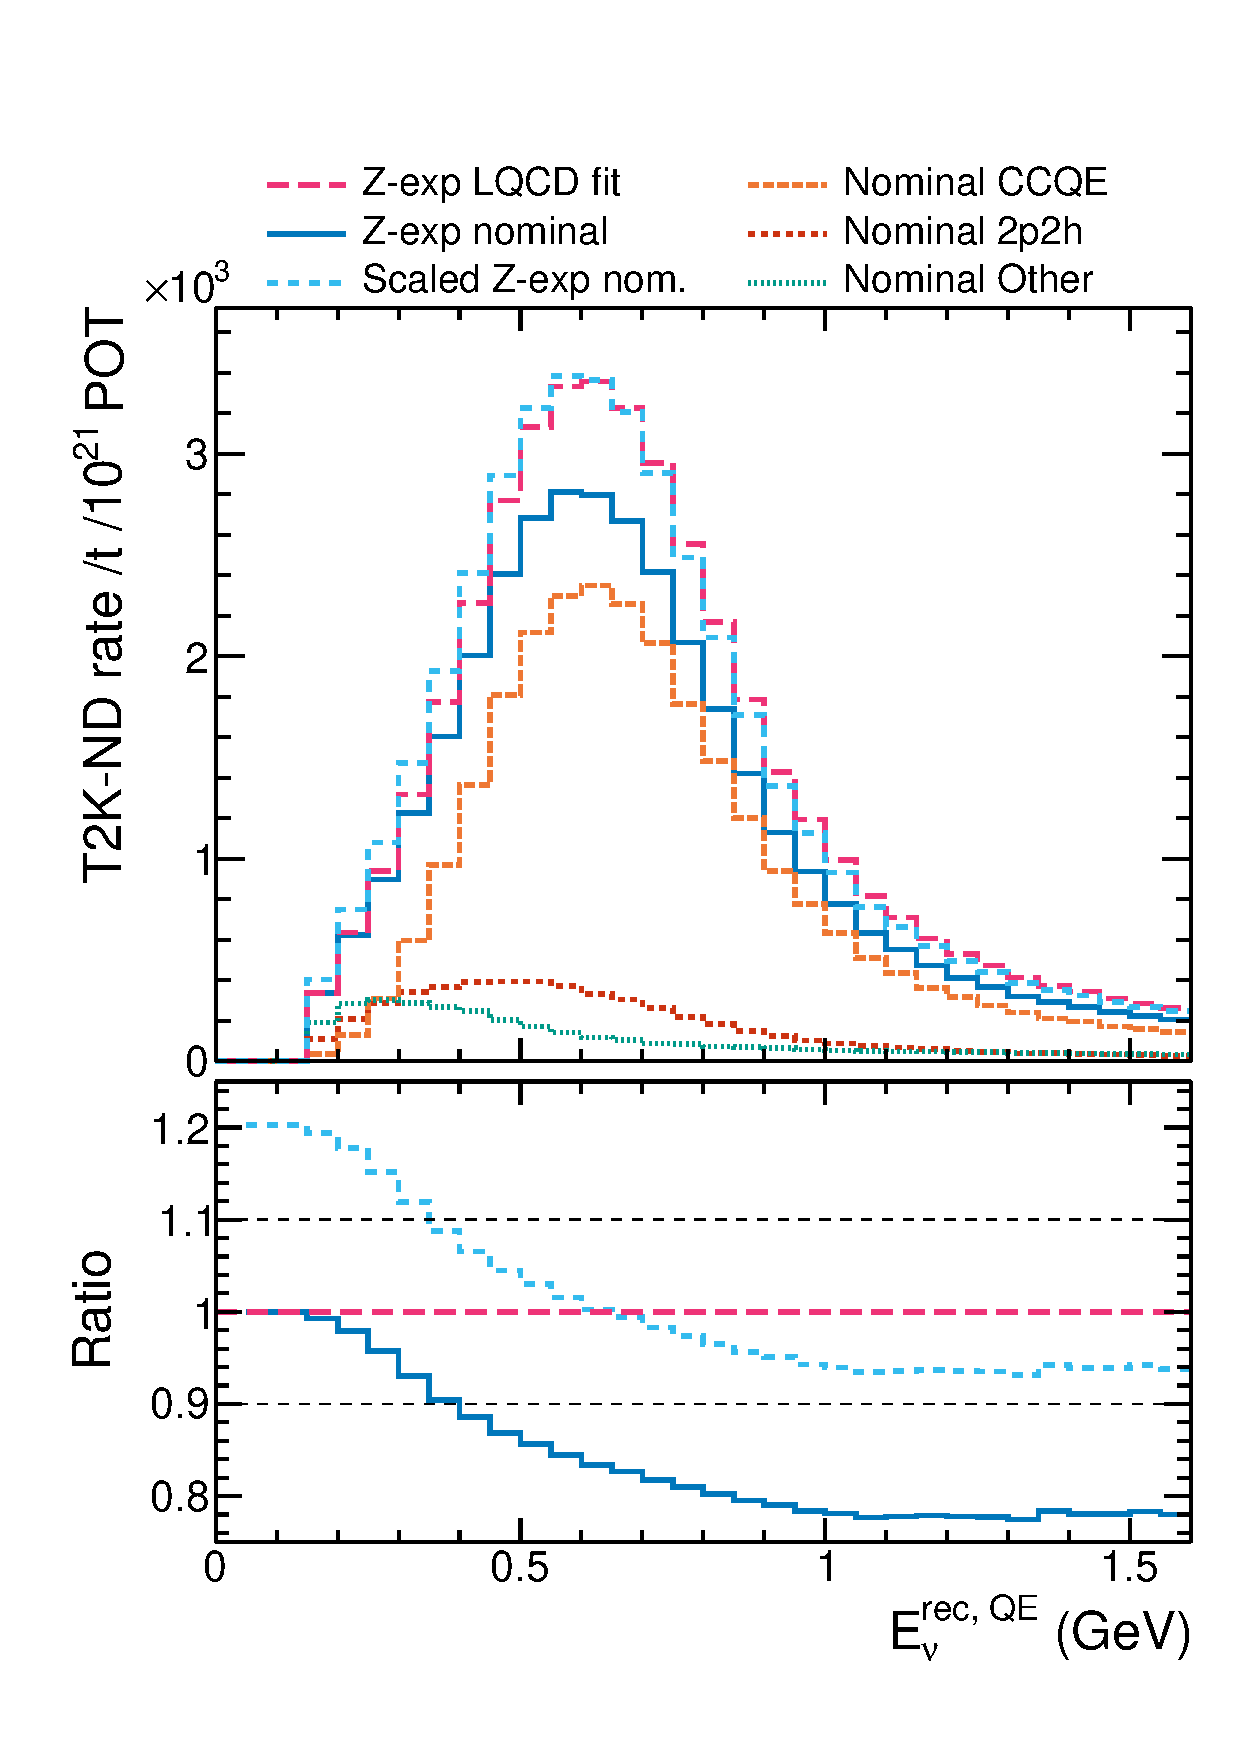
\includegraphics[width=0.3\textwidth]{plots/T2KND_numu_H2O_model_comp.pdf}}\hspace{75pt}
  \subfloat[Far detector] {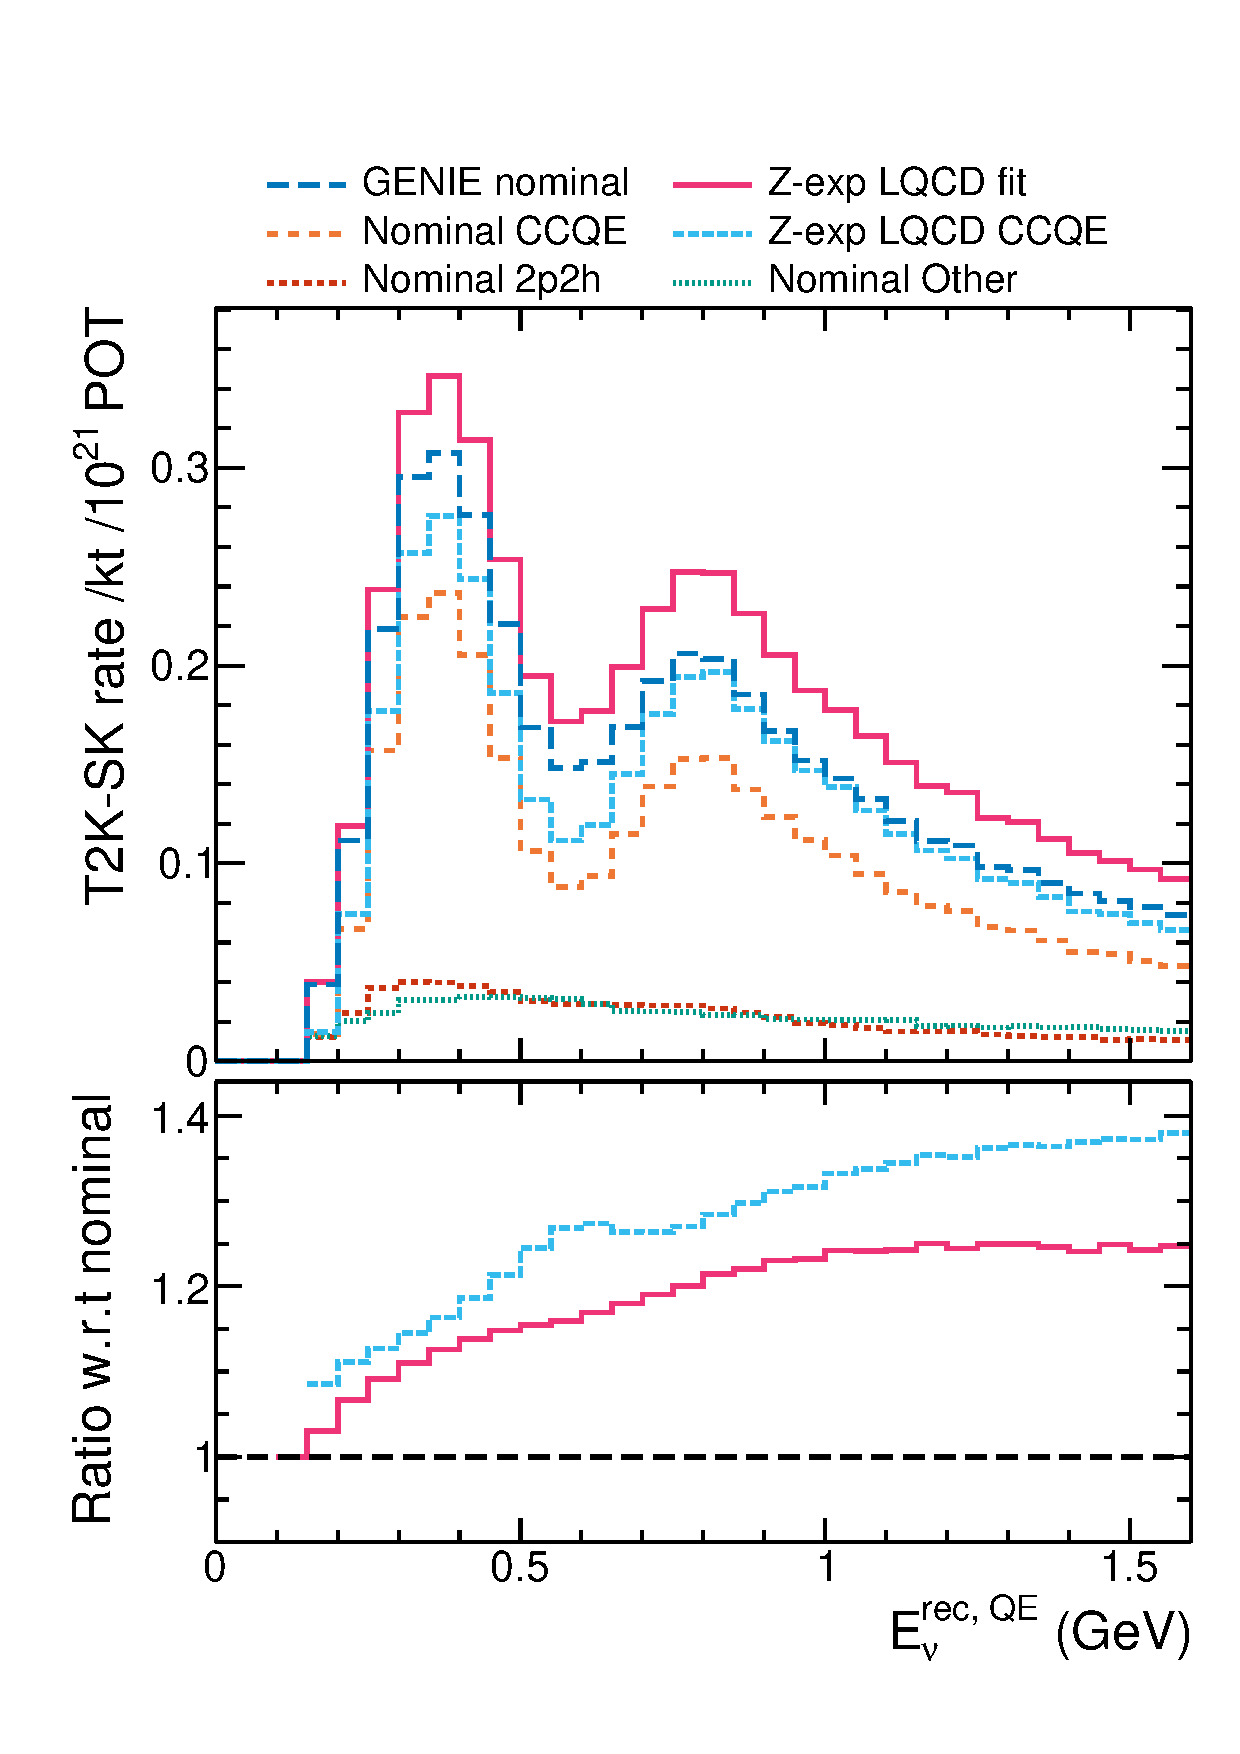
\includegraphics[width=0.3\textwidth]{plots/T2KFD_numu_H2O_osc_model_comp.pdf}}
  \vspace{11pt}
  \caption{The $\nu_{\mu}$--H$_{2}$O CC0$\pi$ event rates per ton (kiloton) per $1\times10^{21}$POT at T2K's near (far) detector site, shown as a function of $E^{\mathrm{rec,\;QE}}_{\nu}$. The GENIE~\cite{Andreopoulos:2009rq, GENIE:2021npt} nominal event rate (blue solid line) is produced using the GENIEv3 10a\_02\_11a tune to nucleon data~\cite{GENIE:2021zuu} and the T2K flux~\cite{T2K:2012bge}, and the CCQE (orange dashed line), CC-2p2h (red short dashed line) and CC-other (green dotted line), here meaning all events that are note CCQE or CC-2p2h, contributions are shown. The oscillated flux is calculated using the best fit NuFit5.0 oscillation parameters in normal ordering~\cite{Esteban:2020cvm, nufitweb}. Additionally, an alternative GENIE model is shown, where the only change is to use the $z$ expansion model of the axial form factor, with parameters tuned to LQCD results from the CalLat collaboration, as described in Section~\ref{sec:callatdata}. Additionally, the ratio of the modified to nominal GENIE models is shown.}
  \label{fig:t2k_impact}
\end{figure}
Figure~\ref{fig:t2k_impact} shows the $\nu_{\mu}$--H$_{2}$O CC0$\pi$ event rate expected at the T2K near and far detectors for a fixed exposure, shown as a function of $E^{\mathrm{rec,\;QE}}_{\nu}\left(p_{l}, \theta_{l}\right)$, with and without modifications to the axial form factor. The nominal GENIEv3 10a\_02\_11a model~\cite{Andreopoulos:2009rq, GENIE:2021npt} uses a dipole axial form factor with $M_{\mathrm{A}} = 0.941$%
\begin{marginnote}
 \entry{$M_{\mathrm{A}}$}{dipole axial mass parameter}
\end{marginnote}%
 GeV obtained through a fit to bubble chamber data~\cite{GENIE:2021zuu}. The alternative model shown differs only in the use of the $z$ expansion model for the axial form factor, with parameters tuned to the LQCD results from the CalLat collaboration described in Section~\ref{sec:callatdata}. One obvious observation to be made from Figure~\ref{fig:t2k_impact} is that the CCQE events which the axial form factor is relevant for clearly make up the majority of T2K's CC0$\pi$ sample, in both the oscillated and unoscillated fluxes. It is also clear that the tuned LQCD values has significant effect on the total expected event rate in both cases, on the order of 20\%.

Also clear from Figure~\ref{fig:t2k_impact} is that the change in the total, or CCQE-contributed event rates is not purely a normalization change, and is different for the near and far detector spectra. In the T2K oscillation analysis, the near detector data is used to constrain the cross section model, to reduce the uncertainty at the far detector and on the measured oscillation parameters. If there is insufficient freedom in the cross section model to account for this change to the CCQE model, other parts of the model may well be distorted to ensure good agreement with the near detector data. However, this can introduce biases at the far detector, as the different interaction types that contribute to the CC0$\pi$ samples shown in Figure~\ref{fig:t2k_impact} have very different $E_{\nu}^{\mathrm{true}}$ --- $E^{\mathrm{rec,\;QE}}_{\nu}$ relationships. So if other components of the model are distorted to fit the unoscillated near detector event rate, that same {\it effective} change is not in general expected to extrapolate to the far detector spectrum correctly.

Experiments with higher neutrino beam energies typically do not limit their analyses to CC0$\pi$ events or use Equation~\ref{eq:enuqe} for reconstructing the neutrino energy. Instead, they use all charged-current events (CC-inclusive), and reconstruct the neutrino energy through a combination of particle identification and tracking, and calorimetry. For an ideal detector, with no tracking threshold on protons, charged pions or electromagnetic activity, this can be expressed as,
\begin{equation}
E_{\nu}^{\mathrm{rec,\;had}} = E_{l} + \Sigma_{p} E_{\mathrm{kin}} + \Sigma_{\pi^{\pm}, \pi^{0}, \gamma} E_{\mathrm{total}},
\label{eq:enuhad}
\end{equation}
\noindent where $E_{l}$ is the energy of the outgoing charged lepton. The $E_{\nu}^{\mathrm{true}}$ --- $E_{\nu}^{\mathrm{rec,\;had}}$ smearing in this idealized case is due to missing kinetic energy lost to neutrons, and initial state nuclear effects (e.g., nucleons are not at rest inside the nucleus). Real detectors have tracking thresholds below which charged particles cannot be reconstructed, which results in additional smearing due to missing the masses of charged pions, although some energy lost to neutrons may be recovered.

\begin{figure}[htbp]
  \centering
  \subfloat[ND]{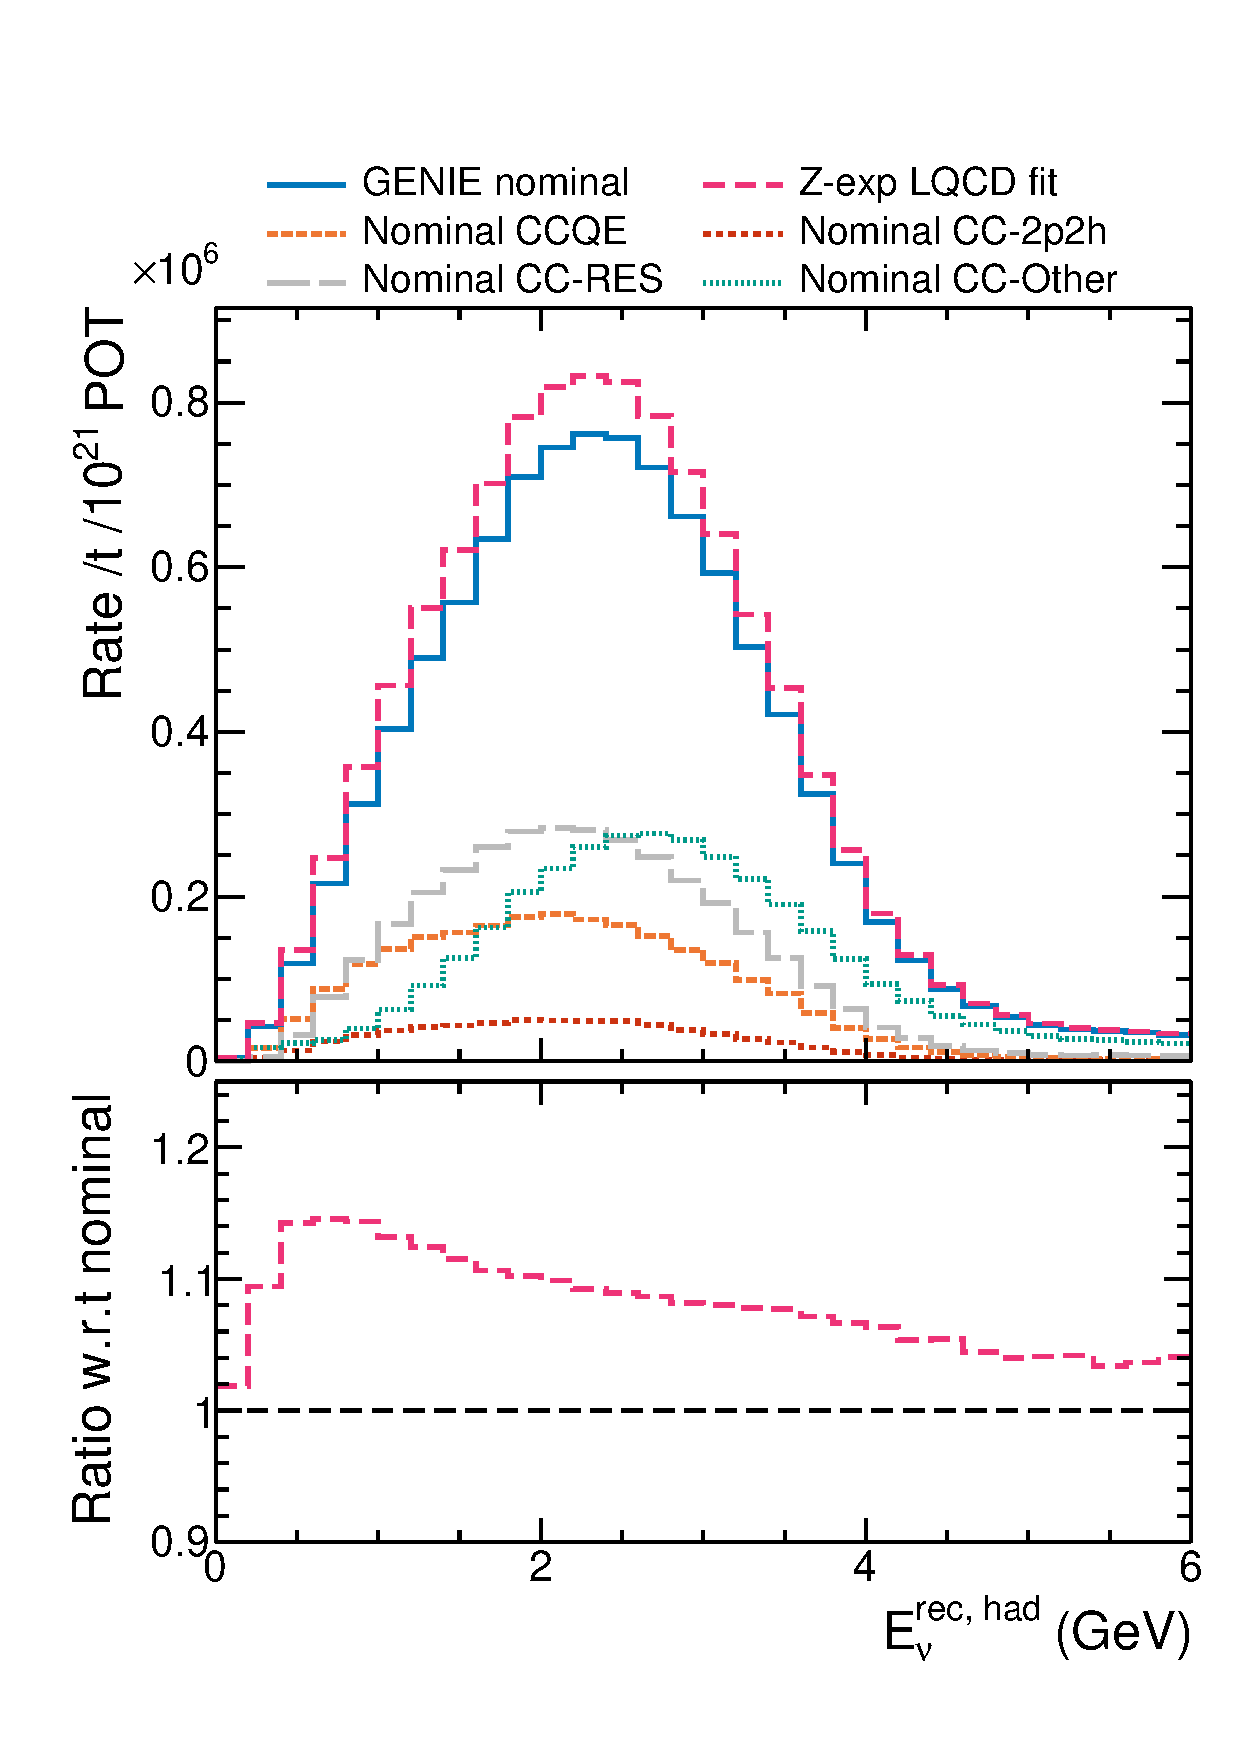
\includegraphics[width=0.3\textwidth]{plots/DUNE_numu_Ar40_breakdown.pdf}}\hspace{75pt}
  \subfloat[FD]{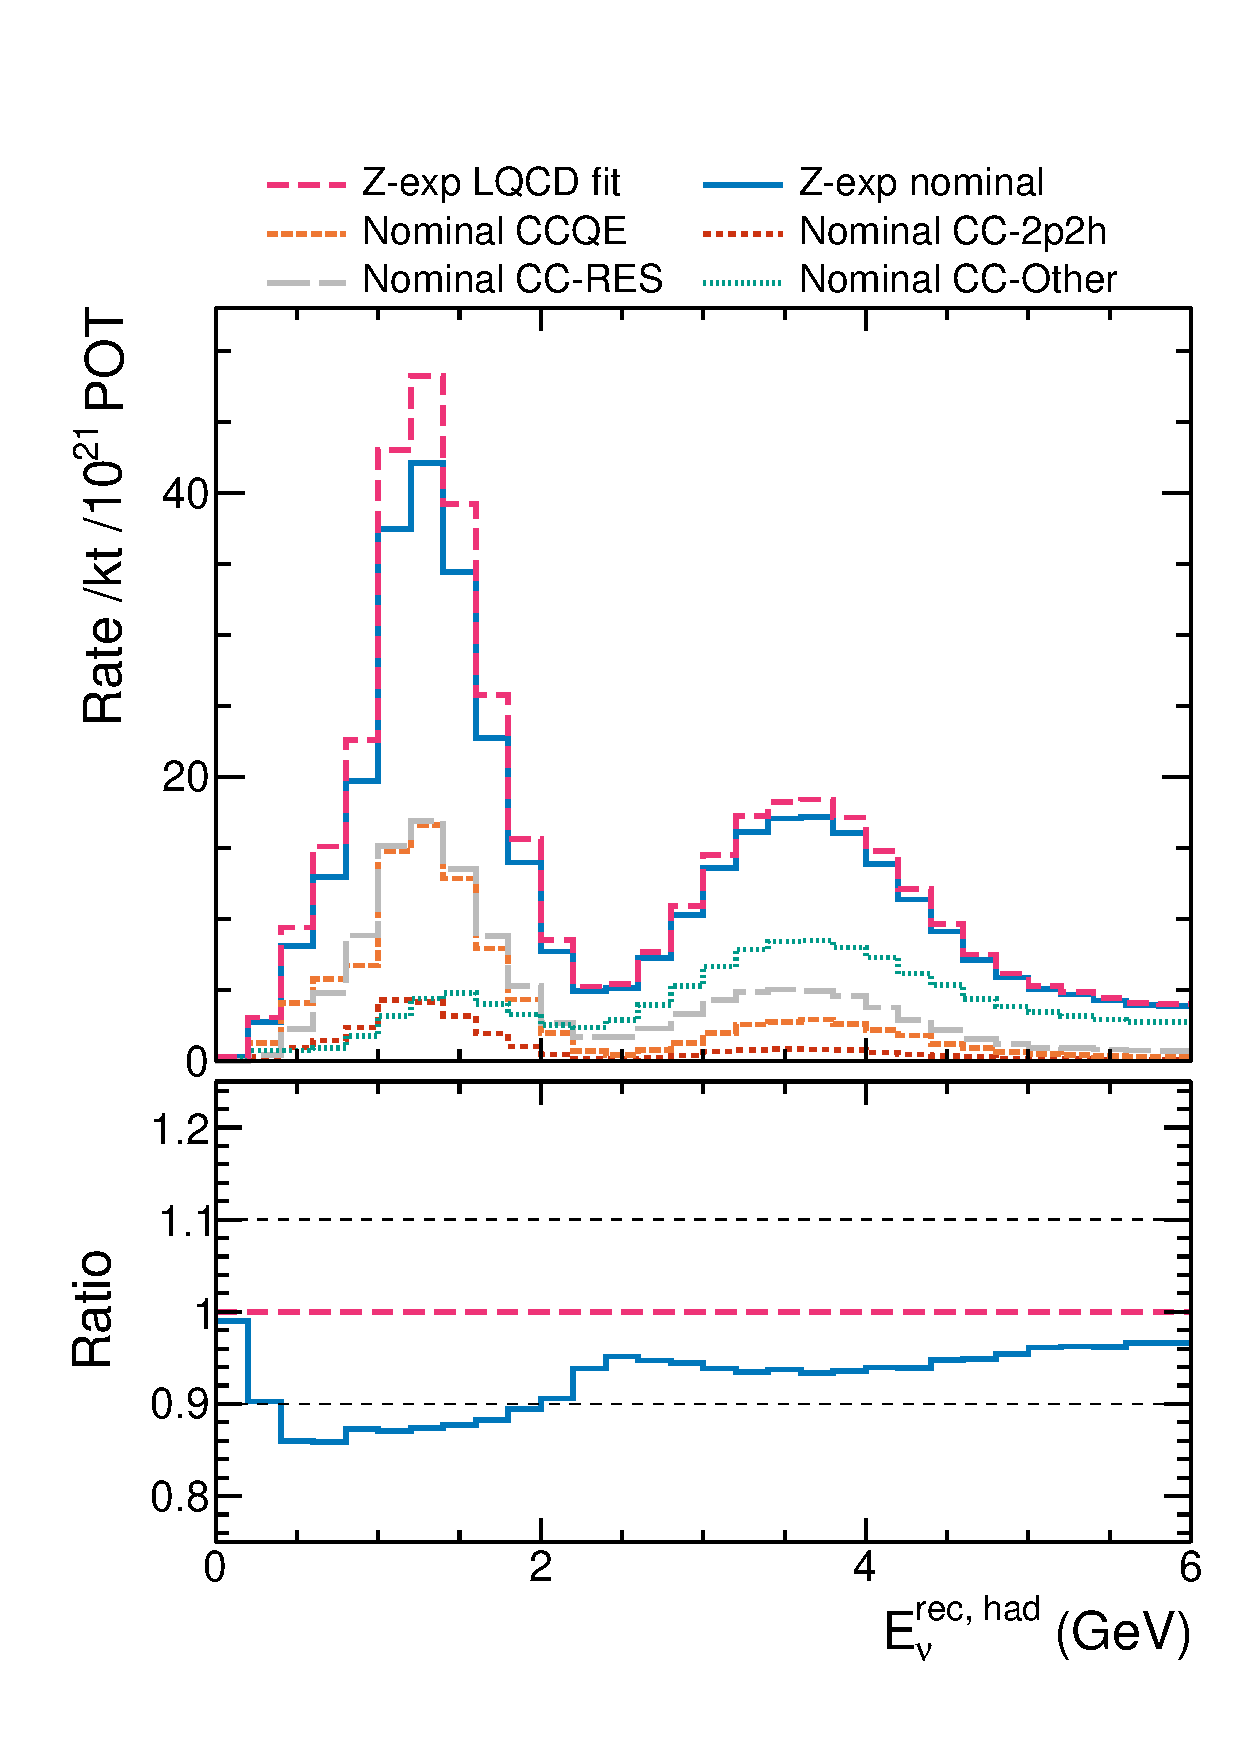
\includegraphics[width=0.3\textwidth]{plots/DUNE_osc_numu_Ar40_breakdown.pdf}}
  \vspace{11pt}
  \caption{The $\nu_{\mu}$--$^{40}$Ar CC-inclusive event rates per ton (kiloton) per $1\times10^{21}$POT at DUNE's near (far) detector site, shown as a function of $E^{\mathrm{rec,\;had}}_{\nu}$. The GENIE~\cite{Andreopoulos:2009rq, GENIE:2021npt} nominal event rate (blue solid line) is produced using the GENIEv3 10a\_02\_11a tune to nucleon data~\cite{GENIE:2021zuu} and the DUNE flux~\cite{Abi:2020evt}, and the CCQE (orange dashed line), CC-2p2h (red short dashed line), CC-RES (long-dashed gray line) and CC-other (green dotted line), here meaning all events that are not CCQE, CC-2p2h or CC-RES, contributions are shown. The oscillated flux is calculated using the best fit NuFit5.0 oscillation parameters in normal ordering~\cite{Esteban:2020cvm, nufitweb}. Additionally, an alternative GENIE model is shown, where the only change is to use the $z$ expansion model of the axial form factor, with parameters tuned to LQCD results from the CalLat collaboration, as described in Section~\ref{sec:callatdata}. Additionally, the ratio of the modified to nominal GENIE models is shown.}
  \label{fig:dune_impact}
\end{figure}
Figure~\ref{fig:dune_impact} shows the $\nu_{\mu}$--$^{40}$Ar CC-inclusive event rates per ton (kiloton) per $1\times10^{21}$POT at DUNE's near (far) detector site, shown as a function of $E^{\mathrm{rec,\;had}}_{\nu}$, with and without modifications to the axial form factor. At this higher neutrino beam energy (with $E_{\nu}^{\mathrm{peak}} \approxeq 2.5$ GeV), CCQE events still make up a sizeable, $\approx$30\%, fraction of the total events. The modification to the axial form factor based on the LQCD results from the CalLat collaboration described in Section~\ref{sec:callatdata} has an approximately 10\% effect to the total predicted event rate at both the near and far detectors, with different shape dependence, as in the T2K case. Despite the different neutrino energy reconstruction methods used by DUNE and T2K, the same arguments about potential bias due to model-dependence apply when there are differences in the effect of an out-of-model change between near and far detectors.

The issue of how to assign strength between the CCQE and CC-2p2h channels has been a major focus for neutrino oscillation experiments over the past decade. Experimental data from a large number of experiments has found disagreements on the 10--30\% level between model predictions and data in the CC$0\pi$ channel~\cite{garvey_review_2014, Mosel:2016cwa, NuSTEC:2017hzk, Katori:2016yel, ParticleDataGroup:2020ssz}, prompting development of {\it ad hoc} systematic uncertainties and empirical model tunings by individual experiments, with a tendancy has been to soak up model-data discrepancies into the CC-2p2h channel. These are major contributors to the final uncertainties on key oscillation parameter measurements and projected sensitivities~\cite{T2K:2019bcf, DUNE:2020jqi, T2K:2021xwb, NOvA:2021nfi, DUNE:2021mtg}. It is therefore very significant that the LQCD results shown in Figures~\ref{fig:t2k_impact} and~\ref{fig:dune_impact} suggest that an increase to the strength of the CCQE contribution on the order of 20\% is necessary.


% ------------------------------------------------------------------------------
% Future
\section{Future Improvements\label{sec:future}}

The most pressing issue \change{that needs to be} definitively \change{resolved for} the LQCD calculations is whether or not the excited state contamination is under complete control for the nucleon (quasi-)elastic form factor calculations.
If they are, then the LQCD results indicate that the nucleon axial form factor is significantly different than what has been extracted phenomenologically, as indicated in Figure~\ref{fig:gaq2_overlay}.
However, it is worth observing that LQCD calculations of $g_{\mathrm{A}}$ were systematically low for many years, before it was finally understood the issues was related to an under-estimation of the systematic uncertainty associated with these excited states.

There are several groups computing these form factors, with several different lattice actions and several different approaches to quantifying and removing the excited state contamination from the ground state matrix elements.
Given the heightened awareness of this issue, it is much less likely that all the LQCD results are polluted by such a contamination than was the case for $g_{\mathrm{A}}$.
The most clear way to definitively resolve the question would be to perform an extremely high statistics calculation with source-sink separation times of $\tsep\approx$2--3~fm.  The extreme numerical cost
renders this an unlikely approach.
In the longer term, the use of multi-level integration schemes can lead to an exponentially improved stochastic precision~\cite{Ce:2016idq}.

A much more practical solution presently would be to implement a variational calculation using distillation~\cite{HadronSpectrum:2009krc} or its stochastic variant~\cite{Morningstar:2011ka}.
There are several advantages to such a calculation.
First, these methods enable the use of multi-hadron creation and annihilation operators
 that are essential to properly identify both the spectrum and the nature of the state~\cite{Dudek:2012xn,Lang:2012db},
 whether it is a $P$-wave $N\pi$ state,
 some radial excitation of the nucleon such as the Roper
 which can prominantly decay to an $N\pi\pi$ state,
 or otherwise.
Given this information, one can construct linear combinations of these operators which systematically remove the excited states from the correlation function~\cite{Blossier:2009kd}, allowing for the utilization of much earlier Euclidean times where the stochastic noise is relatively much smaller.
Second, these variational methods enable the use of momentum space creation as well as annihilation operators, with full control over the spin projection of the source and sink at minimal extra cost.
This enables one to construct useful linear combinations of correlation functions that eliminate for example, the induced pseudoscalar contribution to an axial three point function, simplifying the analysis~\cite{Meyer:2017ddy}.
Further, one can exploit the Breit-Frame in which magintude of the incoming and outgoing momentum are the same which opens the door for utilizing the Feynman-Hellmann-like correlation functions which suppress the excited state contamination significantly compared to the three-point functions~\cite{He:2021yvm}.
It is encouraging that the first exploratory calculations with such methods have begun~\cite{Egerer:2018xgu,Barca:2021iak}.

Given the state of the field and the rapid advances recently made, we anticipate this excited state issue will be definitively resolved for elastic nucleon form factor calculations within a year or two, thus enabling precise determinations of the quasi-elastic axial form factor and the elastic electric and magnetic form factors that will resolve the discrepancies reviewed in Section~\ref{sec:sof}.


Moving beyond these simplest quantities, higher energy transfer processes also play a sub-dominant role for T2K (and the future
Hyper-K) experiments, and a major role in the DUNE experiment which has a higher energy neutrino
flux, as can be seen in Figures~\ref{fig:t2k_impact} and~\ref{fig:dune_impact}, respectively.
These higher energy transfers can access other fundamentally different interaction topologies,
 such as resonant or nonresonant pion production mechanisms,
 nuclear responses with correlated nucleon pairs,
 or scattering off partons within nucleons.
In principle, all of these interaction mechanisms are accessible to LQCD,
 though with varying degrees of difficulty.
Given the discrepancy between lattice axial form factor data and experimental constraints,
 it is not unreasonable to expect other interaction mechanisms have similar discrepancies
 between theory and observation.
These interaction types are as inaccessible as CCQE with modern $\nu A$ data, typically relying on old H$_2$ and D$_2$ bubble chamber datasets, with even lower statistics than the historic CCQE datasets already discussed, compounding the problem.
Appeals to model assumptions may give some handle for missing quantities,
 but are also subject to unquantifiable systematic effects.

Calculations that access the combined resonant and nonresonant scattering amplitudes
 are the most similar to those of elastic scattering,
 where a current induces a transition of the nucleon to a multiparticle final state.
The most prominent resonant contribution is from the $N\rightarrow\D$ transition.
However, building up an understanding of the entire resonant region, following the standard LQCD computational strategy, will be an extremely challenging endeavour given the dense spectrum of multi-particle states, and more importantly, the lack of formalism to relate three-particle matrix elements in finite volume to the infinite volume physics of interest.
It is likely that alternative strategies which focus on the inclusive $N\rightarrow X$ contribution~\cite{Hansen:2017mnd,Gambino:2020crt,Fukaya:2020wpp,Bruno:2020kyl}, or the use of two-currents to compute the hadronic tensor~\cite{Liu:1993cv,Liang:2019frk} will be more fruitful.

Calculations of two-nucleon matrix elements provide key insights
 about the correlations between nucleons inside a nuclear medium,
 a vital ingredient for construction of an effective theory
 of $\nu A$ interactions.
The first efforts have been made to compute two-nucleon matrix elements in response to electroweak currents~\cite{Savage:2016kon,Chang:2017eiq}.
These calculations will most likely have to be revisited with a variational method as well,
 since it now appears the use of local two-nucleon creation operators do not correctly
 reproduce the spectrum~\cite{Francis:2018qch,Horz:2020zvv,Green:2021qol,Amarasinghe:2021lqa}.
Future calculations of matrix elements for currents inserted between
 two-nucleon states could provide direct information about the LEC inputs to EFT descriptions of nuclear physics.
While EFT can not be used to describe the $\nu A$ response over the full kinematic range of interest, they can provide a crucial anchor point to constrain nuclear models, see for example Refs.~\cite{Kronfeld:2019nfb,Drischler:2019xuo,Tews:2020hgp,Davoudi:2020ngi}
As a specific example, deuterium corrections from nuclear models were assumed to be strong only at low momentum transfer
 and energy-independent in the reanalysis of deuterium bubble chamber data~\cite{Meyer:2016oeg},
 despite the inability of these corrections to account for the theory-data discrepancies.
A direct LQCD computation of these effects would isolate the effect,
 either by definitively attributing the discrepancy to deuterium effects
 or by implicating the other systematics corrections.


% ------------------------------------------------------------------------------
% Conclusions
\section{Conclusions\label{sec:conclusions}}

LQCD collaborations are able to produce consistent results for benchmark quantities such as $g_{\mathrm{A}}$ with percent level systematic uncertainties, which are in excellent agreement with experimental data.
These results introduce the exciting possibility of LQCD calculations to tackle other quantities that are not easily experimentally accessible, or for which tensions between measurements, or competing models, exist.
In this review we discussed using LQCD to calculate nucleon form factors as a function of momentum transfer, which are of particular interest to the few-GeV neutrino experimental program.
Notable tensions exist in current parameterizations of the vector form factors, but here we focused on the axial form factor, $F_{\mathrm{A}}(Q^2)$, which is of primary importance because current parameterizations are simplistic and rely on a handful of low-statistics $\nu N$ bubble chamber measurements.
$F_{\mathrm{A}}(Q^2)$ cannot be cleanly measured with existing experiments which use heavier nuclear targets both for safety reasons and to increase the event rate, so LQCD offers a novel path to this important quantity.
We have compared $F_{\mathrm{A}}(Q^2)$ calculations from a variety of different LQCD collaborations using different approaches and techniques, and shown them to be in good agreement with each other, but crucially, in poor agreement with the simple dipole model tuned to historic $\nu N$ data currently relied upon.
Assuming that no systematic effects affecting all of the LQCD calculations are uncovered, this suggests a significant increase of approximately 20\% to the strength of the CCQE scattering channel that dominates the neutrino scattering cross section for $E_{\nu} \lesssim 1$ GeV.
We have demonstrated that these results produce a significant change in the predicted neutrino event spectra for T2K (which has similar considerations to Hyper-K) and DUNE experiments.
Determining the impact on oscillation results would require a full analysis performed by each experimental collaboration, but it is clear that LQCD results for $F_{\mathrm{A}}(Q^2)$ may offer a valuable insight that can clarify aspects of the complex neutrino interaction modeling problem these experiments face.
We additionally discussed a number of ways in which current calculations can be improved and validated, and to increase confidence that the LQCD results are not subject to an uncontrolled systematic uncertainty.
Finally, we discussed a number of other quantities that are important to neutrino oscillation experiments in the few-GeV energy regime that LQCD can provide first principles predictions for.
These include resonant pion production at higher energy transfers (of particular interest to DUNE), and insights into nucleon-nucleon correlations, for which there are no clear experimental prospects.
These possibilities would all work to break current degeneracies between $\nu N$ interactions and various nuclear effects that all come into play for present modeling efforts of the $\nu A$ cross sections.



%Disclosure
\section*{DISCLOSURE STATEMENT}
While the authors collaboration affiliations do not affect the objectivity of this review, we wish to include them for transparency. ASM and AWL are both current members of the CalLat collaboration. ASM is a current member of the Fermilab Lattice and MILC collaborations. CW is a current member of the T2K and DUNE collaborations.
The authors are not aware of any funding, or financial holdings that might be perceived as affecting the objectivity of this review.

% Acknowledgements
\section*{ACKNOWLEDGMENTS}
The work of ASM was supported by the Department of Energy, Office of Nuclear Physics, under Contract No. DE-SC00046548.
The work of AWL and CW was supported by the Director, Office of Science, Office of Basic Energy Sciences, of the U.S. Department of Energy under Contract No. DE-AC02-05CH11231.


% References
\bibliography{AR_review.bib}
\bibliographystyle{ar-style5}
%ArXiv references may be formatted as follows, in the Literature Cited section: “1. Author A, Author B. arXiv:XXXX.XXXX [hep-ph] (2017)”

\end{document}
